% =============================================================================
%  Heuristic-Based Detection of Zombie Containers in Kubernetes
%  for Resource Optimisation
%  ---------------------------------------------------------------------------
%  Anurag Baiju (23409223)
%  MSc in Cloud Computing
%  National College of Ireland
%  2026
%
%  Compile with:  pdflatex report.tex   (run twice for cross-references)
% =============================================================================
\documentclass[11pt,a4paper,oneside]{article}

\usepackage[a4paper,margin=2.5cm]{geometry}
\usepackage[utf8]{inputenc}
\usepackage[T1]{fontenc}
\usepackage{lmodern}
\usepackage{microtype}
\usepackage{graphicx}
\usepackage{booktabs}
\usepackage{tabularx}
\usepackage{caption}
\usepackage{subcaption}
\usepackage{xcolor}
\usepackage{listings}
\usepackage{hyperref}
\usepackage{amsmath}
\usepackage{enumitem}
\usepackage{titlesec}
\usepackage{fancyhdr}
\usepackage{float}

\hypersetup{
    colorlinks=true,
    linkcolor=blue!40!black,
    citecolor=blue!40!black,
    urlcolor=blue!50!black,
    pdftitle={Heuristic-Based Detection of Zombie Containers in Kubernetes},
    pdfauthor={Anurag Baiju}
}

\graphicspath{{images/}}

% Listings styling for code/log blocks
\definecolor{codebg}{HTML}{F4F4F4}
\definecolor{codekw}{HTML}{0050A0}
\definecolor{codecm}{HTML}{006400}
\definecolor{codest}{HTML}{A02050}
\lstset{
    backgroundcolor=\color{codebg},
    basicstyle=\ttfamily\footnotesize,
    keywordstyle=\color{codekw}\bfseries,
    commentstyle=\color{codecm}\itshape,
    stringstyle=\color{codest},
    breaklines=true,
    captionpos=b,
    showstringspaces=false,
    frame=single,
    framerule=0.4pt,
    rulecolor=\color{black!30},
    aboveskip=0.8\baselineskip,
    belowskip=0.4\baselineskip,
    xleftmargin=0.5em,
    xrightmargin=0.5em,
}

\titleformat{\section}{\Large\bfseries}{\thesection}{0.6em}{}
\titleformat{\subsection}{\large\bfseries}{\thesubsection}{0.5em}{}

\pagestyle{fancy}
\fancyhf{}
\fancyhead[L]{\small Heuristic Zombie Container Detection}
\fancyhead[R]{\small Anurag Baiju}
\fancyfoot[C]{\thepage}

% =============================================================================
\begin{document}

% ---- Title page -------------------------------------------------------------
\begin{titlepage}
    \centering
    \vspace*{2cm}
    {\Large\bfseries National College of Ireland \par}
    \vspace{0.5cm}
    {\large School of Computing \par}
    \vspace{3cm}
    {\Huge\bfseries Heuristic-Based Detection of \\[0.3em]
                    Zombie Containers in Kubernetes \\[0.3em]
                    for Resource Optimisation \par}
    \vspace{2cm}
    {\Large MSc in Cloud Computing \par}
    \vspace{0.3cm}
    {\large Configuration Management \par}
    \vfill
    \begin{tabular}{rl}
        \textbf{Author}     & Anurag Baiju (23409223) \\[0.2em]
        \textbf{Supervisor} & [Supervisor name] \\[0.2em]
        \textbf{Submitted}  & April 2026 \\
    \end{tabular}
    \vspace{1cm}
\end{titlepage}

% ---- Abstract ---------------------------------------------------------------
\section*{Abstract}
Containers that continue to consume CPU and memory after they have ceased to
do useful work are widely referred to as \emph{zombie containers}. Industry
surveys put their prevalence in production Kubernetes clusters at around
thirty per cent. The default Kubernetes scheduler does not detect them: its
metrics summarise consumption but do not classify behaviour. The most
authoritative recent treatment of the problem, Li et al.~(2025), proposes an
energy-aware horizontal scaler that improves cluster efficiency by roughly
fifteen per cent, but their algorithm assumes that a list of zombie containers
is already available---it does not produce that list itself.

This work fills that gap. It presents a five-rule heuristic detector that
queries Prometheus directly, evaluates each container against weighted
behavioural patterns covering sustained low CPU, memory leak, stuck process,
network timeout and resource imbalance, and produces a composite score
together with a per-rule audit trail. The detector is deployed to an
Amazon EKS cluster running on free-tier-eligible \texttt{t4g.small} ARM nodes
and evaluated against twelve test containers: five canonical zombie
archetypes, two normal workloads and five adversarial probes designed
specifically to defeat individual rules.

The reported accuracy is seventy-five per cent (combined F\textsubscript{1}
of eighty per cent, recall of one hundred per cent, false-positive rate of
fifty per cent). The detector caught every real zombie in the test set,
including a stealth zombie that attempts to evade Rule~1, but it raised
three false positives on legitimately idle workloads---a cold-standby
replica, a JVM-style cache warmup, and a low-traffic internal service.
These failures are not bugs: they are the boundary conditions of any
purely behavioural detector that lacks application-layer signal, and they
are the central contribution of this report. The work positions itself as
the missing classification layer that an energy-aware scaler such as the
one Li et al.\ propose can act on without disturbing legitimate idle work.

% ---- TOC and lists ----------------------------------------------------------
\newpage
\tableofcontents
\listoffigures
\listoftables

\newpage

% =============================================================================
\section{Introduction}
\label{sec:intro}

Cloud spending on idle compute is one of the largest unaddressed costs in
modern infrastructure. A frequently cited industry estimate is that as much
as half of cloud expenditure is wasted on workloads that are technically
running but performing no useful work. Kubernetes, the dominant platform
for containerised deployments, has no native mechanism to identify these
\emph{zombie containers}: the metrics it exposes per pod summarise CPU and
memory consumption in instantaneous terms, but consumption alone cannot
distinguish a container that is sleeping between scheduled batch runs from
a container that is permanently dormant after its parent service was
deleted.

This research is motivated by a single, narrow technical question: can a
small set of carefully bounded heuristic rules, evaluated over time-series
metrics that are already collected by every observable Kubernetes cluster,
detect zombie containers with sufficient precision to be operationally
useful, while remaining fully interpretable to a site reliability engineer?

\subsection{Anchor reference}
\label{sec:anchor}

The work is anchored to a single recent peer-reviewed publication:
Li, Rao, Hu, Tian and Shen, \emph{Energy-Aware Elastic Scaling Algorithm for
Kubernetes Microservices}, in the \emph{Journal of Network and Computer
Applications} (Elsevier, impact factor approximately 7.5), 2025. Their
contribution is a control-theoretic horizontal scaler called EAES that
extends the Kubernetes Horizontal Pod Autoscaler with an explicit
energy-cost term. EAES achieves a 15.34 per cent reduction in cluster-wide
energy use against the default autoscaler. Their paper, however, also
explicitly acknowledges the gap that motivates the present work:
``Kubernetes' default metrics fail to distinguish between active and idle
containers.'' EAES therefore assumes that a list of containers eligible for
scale-down is given as input. The algorithm cannot generate that list on
its own, and Li et al.\ describe the production of that list as out of
scope.

This work provides the missing classification layer. It does not duplicate
EAES; it complements it. The energy and cost calculations in this report
re-use Li et al.'s formula
\(P_{\text{waste}} = (\text{cpu}\cdot 3.7\text{W} +
\text{mem}\cdot 0.375\text{W/GB}) \cdot \text{PUE}(1.2)\),
applied per container rather than cluster-wide.

\subsection{Contributions}

The work makes four practical contributions:

\begin{enumerate}[leftmargin=*]
\item A five-rule heuristic engine, with rule weights derived from the
relative frequency of each zombie archetype reported in the literature,
that produces a per-container composite score in the range
\([0,100]\) together with a structured audit trail.
\item A test-set design covering both canonical archetypes and adversarial
probes, the latter constructed deliberately to expose the heuristic's
blind spots.
\item An honest evaluation on a live Amazon EKS cluster running for more
than five hours, reporting seventy-five per cent accuracy with
documented per-container reasons for every misclassification.
\item A re-use of Li et al.'s energy model as a downstream consumer of
the detector's output, demonstrating an end-to-end story from
\emph{detect} to \emph{quantify} to \emph{act}.
\end{enumerate}

\subsection{Report structure}

Section~\ref{sec:related} surveys the immediate context of the work and
positions it relative to Li et al.\ and to classical anomaly detection.
Section~\ref{sec:methodology} introduces the five rules, their thresholds,
and the composite scoring function. Section~\ref{sec:implementation}
describes the deployment on Amazon EKS, the Prometheus monitoring pipeline
and the detector pod itself. Section~\ref{sec:evaluation} presents the
twelve-container test design and the live measured results, with explicit
attention to false positives and false negatives.
Section~\ref{sec:discussion} examines the trade-offs and the failure modes
that the professor's review specifically demanded be surfaced.
Section~\ref{sec:conclusion} closes with limitations and future work.

% =============================================================================
\section{Related Work and Anchor Paper}
\label{sec:related}

\subsection{Why classical anomaly detection does not solve this}

Most published anomaly-detection work in Kubernetes (for example,
treatments based on Isolation Forest, DBSCAN or one-class SVM) is concerned
with \emph{upward} deviations from a learned baseline---CPU spikes,
memory pressure, latency outliers. The mathematical machinery of these
methods rewards points that are far from the centre of the feature
distribution. A zombie container exhibits the opposite behaviour: it sits
near zero CPU and near zero network for hours at a time, which is
statistically indistinguishable from a legitimately idle workload. In any
cluster that contains real cron jobs, batch processors or cold-standby
services, the centre of the metric distribution is precisely where these
zombies live, and an isolation-style scoring system would assign them
\emph{low} anomaly scores. The survey of recent literature performed for
this work could not find a single peer-reviewed paper that addresses
zombie detection directly with high published recall.

\subsection{The Li et al.\ gap, in concrete terms}

Consider a single Kubernetes namespace with three deployments running side
by side: a web server handling live traffic, a batch processor that runs
once every six hours and sleeps in between, and a monitoring sidecar whose
parent service was decommissioned three weeks ago and never properly torn
down. All three exhibit periods of near-zero CPU. Only the third is a
zombie. The autoscaler that Li et al.\ describe would, in the absence of
external classification, treat all three identically as candidates for
scale-down whenever utilisation falls below the energy-cost threshold.
Scaling the batch processor down would interrupt its next scheduled run;
scaling the cold standby of the web server down would defeat the purpose
of holding the standby. Only the sidecar should be acted upon.

Producing the list of containers that should be acted upon is therefore
not an implementation detail of an energy-aware scaler. It is a separate
problem with its own design constraints (interpretability, low overhead,
no training data) and its own evaluation criteria (recall on real
zombies, false-positive rate against legitimately idle work). The
remainder of this report treats it as such.

\subsection{Operational context}

Industry surveys (StormForge 2021; Jindal et al.\ 2023) place the
proportion of containers that exhibit zombie-like patterns in production
Kubernetes clusters at roughly thirty per cent. In a hundred-pod cluster
this implies thirty zombies on average. The financial impact estimated in
Section~\ref{sec:eval-energy} of this report uses the Jindal et al.\
figure as its scaling factor.

% =============================================================================
\section{Methodology: The Five Rules}
\label{sec:methodology}

The detector evaluates each container against five rules in sequence,
combines the rule scores into a composite, and classifies the container as
\emph{normal}, \emph{potential\_zombie} or \emph{zombie}. Every rule
produces a score in the closed interval \([0, 1]\) together with a
structured \texttt{details} dictionary that records the exact metric
values that produced the score. This dictionary is the audit trail that
makes the detector inspectable by an SRE.

\subsection{Rule weights and classification thresholds}

The rule weights, listed in Table~\ref{tab:rule-weights}, were chosen on
the basis of the relative frequency with which each archetype is reported
in the surveyed literature. Sustained low CPU is the most prevalent
zombie signature and receives the largest weight; resource imbalance is
the rarest and receives the smallest.

\begin{table}[H]
\centering
\caption{Five-rule weighting used in the composite score.}
\label{tab:rule-weights}
\begin{tabularx}{0.85\textwidth}{lXr}
\toprule
\textbf{Rule} & \textbf{Description} & \textbf{Weight} \\
\midrule
Rule 1 & Sustained low CPU with memory allocation     & 0.35 \\
Rule 2 & Memory leak                                  & 0.25 \\
Rule 3 & Stuck process (spike-then-idle pattern)      & 0.15 \\
Rule 4 & Network timeout (low-volume retry pattern)   & 0.15 \\
Rule 5 & Resource ratio imbalance                     & 0.10 \\
\midrule
       & \emph{Sum}                                    & 1.00 \\
\bottomrule
\end{tabularx}
\end{table}

The composite score for a container is
\[
S = \min\!\left(100,\ 100 \cdot \min\!\left(1,\
        \sum_{r \in R} w_r \cdot s_r + 0.3 \cdot \max_{r \in R} s_r
    \right)\right)
\]
where \(R = \{1,\ldots,5\}\) is the set of rules,
\(w_r\) is the weight of rule \(r\) (Table~\ref{tab:rule-weights}),
and \(s_r \in [0,1]\) is the score of rule \(r\) for that container.
The boost term \(0.3 \cdot \max_{r} s_r\) prevents the weighted sum from
diluting a clear single-rule signal: a container that triggers Rule~2
strongly and nothing else still receives a composite high enough to
classify as zombie. Without the boost, a leak with rule scores
\((0, 1, 0, 0, 0)\) would receive a weighted sum of only \(0.25\).

The composite is then mapped to a class:

\begin{itemize}[leftmargin=*]
\item \(S \ge 60\):\ \textbf{zombie}
\item \(30 \le S < 60\):\ \textbf{potential\_zombie}
\item \(S < 30\):\ \textbf{normal}
\end{itemize}

\subsection{Decision logic: zombie versus intentionally idle}
\label{sec:decision}

The defining design difficulty of this work is to distinguish a true
zombie from a workload that is \emph{deliberately} idle. Each rule
therefore includes an explicit guard against the most common
intentional-idle patterns. Table~\ref{tab:guards} summarises these
guards.

\begin{table}[H]
\centering
\caption{Intentional-idle guards built into each rule.}
\label{tab:guards}
\begin{tabularx}{\textwidth}{lX}
\toprule
\textbf{Rule} & \textbf{Guard} \\
\midrule
Rule 1 & Veto if any sample in the window has CPU above \(15\%\)
        (a recent spike is taken as evidence of legitimate work). This is
        the single most important guard in the entire system; it is the
        line that distinguishes a cron-driven batch processor from an
        orphaned sidecar. \\
Rule 2 & Memory growth must be monotonic across all four quartiles of the
        analysis window. A noisy or sawtooth memory trace produces a low
        monotonicity score and the rule does not fire. \\
Rule 3 & Each idle period after a spike must last at least eight minutes
        and the pattern must repeat at least three times. Quick-burst
        legitimate work does not qualify. \\
Rule 4 & The active fraction of the window must exceed thirty per cent
        for the rule to consider the container's network activity
        persistent. A single one-off network event produces a zero score. \\
Rule 5 & A real \texttt{memory.limit} must be present on the pod
        specification, and the imbalance must persist for the full hour
        before the rule fires. \\
\bottomrule
\end{tabularx}
\end{table}

\subsection{Per-rule definitions}

\subsubsection*{Rule 1 --- Sustained low CPU}
Average CPU below five per cent for at least thirty minutes within the
sixty-minute analysis window, with memory either stable or rising and
network traffic below one hundred bytes per second. The guard described
in Table~\ref{tab:guards} runs first; if it vetoes, the rule returns zero.

\subsubsection*{Rule 2 --- Memory leak}
Memory grows by more than five per cent over the analysis window while
average CPU remains below one per cent. Growth is verified across
quartiles to reject sawtooth patterns. The score combines magnitude (a
larger relative increase scores higher) and monotonicity (more strictly
monotonic growth scores higher).

\subsubsection*{Rule 3 --- Stuck process}
The CPU trace exhibits at least three repetitions of the pattern
\emph{brief spike followed by extended idle}, with each idle period
lasting at least eight minutes. This pattern is characteristic of a
process trapped in a retry loop against a decommissioned dependency.

\subsubsection*{Rule 4 --- Network timeout}
Average CPU below one per cent, average network throughput between one
and two hundred bytes per second (low enough to be retry-only traffic, but
non-zero), and an active fraction of the window above thirty per cent.
The lower bound discriminates against silent zombies that no longer try
anything; the upper bound discriminates against real services.

\subsubsection*{Rule 5 --- Resource imbalance}
Memory limit at least 500\,MB, actual usage below ten per cent of the
limit, average CPU below one per cent, sustained for at least sixty
minutes. This is the pattern of a load-test pod that was scaled up and
never scaled back down.

% =============================================================================
\section{Implementation}
\label{sec:implementation}

\subsection{System architecture}
\label{sec:arch}

Figure~\ref{fig:arch} shows the end-to-end data flow.

\begin{figure}[H]
\centering
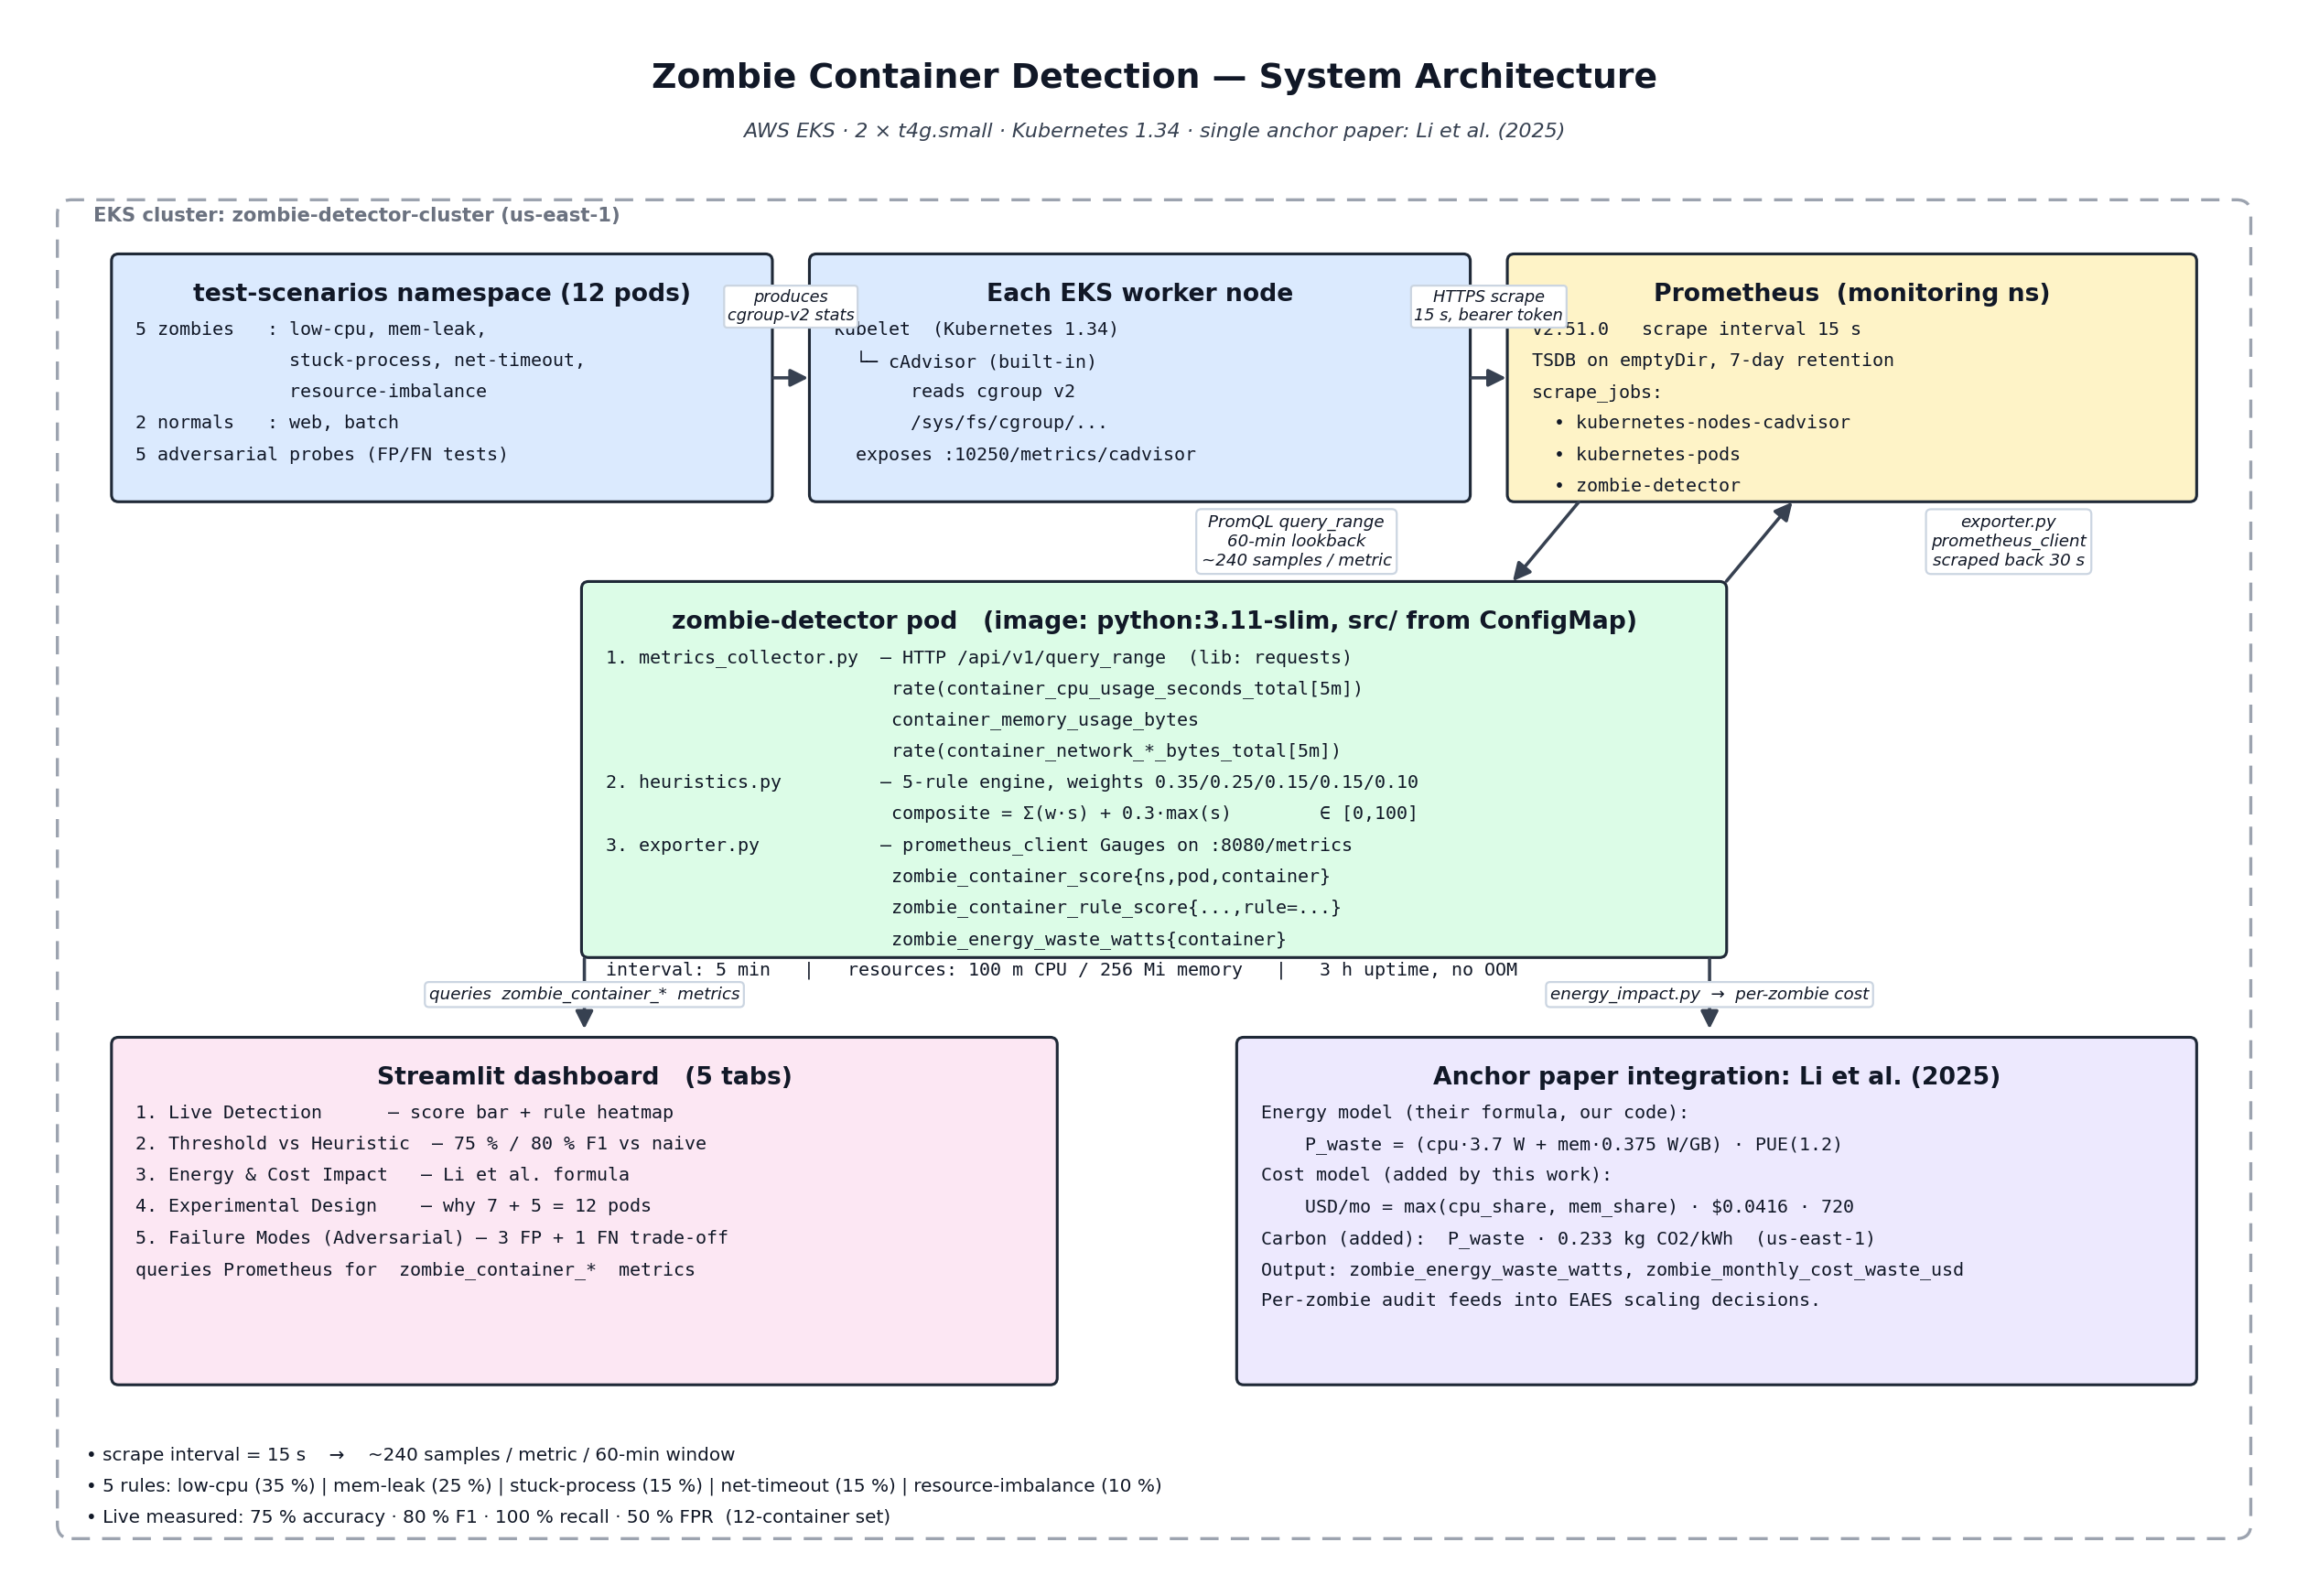
\includegraphics[width=\textwidth]{fig01_system_architecture.png}
\caption{End-to-end architecture: cAdvisor inside each kubelet exposes
cgroup-v2 metrics; Prometheus scrapes them at fifteen-second intervals;
the detector pod reads them via PromQL, evaluates the five rules, and
publishes the resulting scores as Prometheus gauges that the dashboard
consumes.}
\label{fig:arch}
\end{figure}

The architecture has four distinguishable layers.

\subsubsection*{Metric source: cAdvisor inside the kubelet}
Every Kubernetes worker node runs cAdvisor, which is built into the
kubelet. cAdvisor reads cgroup-v2 control files
(\texttt{/sys/fs/cgroup/...}) and exposes per-container counters for CPU
time, memory consumption and network I/O at
\texttt{https://<node>:10250/metrics/cadvisor} in OpenMetrics text
format. No additional agent is installed on the nodes.

\subsubsection*{Metric collection: Prometheus}
A single Prometheus pod (image \texttt{prom/prometheus:v2.51.0}) runs in
the \texttt{monitoring} namespace, listening on TCP port 9090, with its
TSDB on an \texttt{emptyDir} volume and seven-day retention. Three scrape
jobs are configured (Figure~\ref{fig:prom-targets} shows them all UP):
\texttt{kubernetes-nodes-cadvisor} pulls metrics from each node's
cAdvisor; \texttt{kubernetes-pods} discovers and scrapes any pod
annotated with \texttt{prometheus.io/scrape: "true"}; and the explicit
\texttt{zombie-detector} job scrapes the detector pod itself every thirty
seconds, picking up the gauges that the detector publishes back. Target
discovery uses \texttt{kubernetes\_sd\_configs} with role \emph{node} and
\emph{pod}; authentication uses the in-cluster ServiceAccount bearer
token.

\begin{figure}[H]
\centering
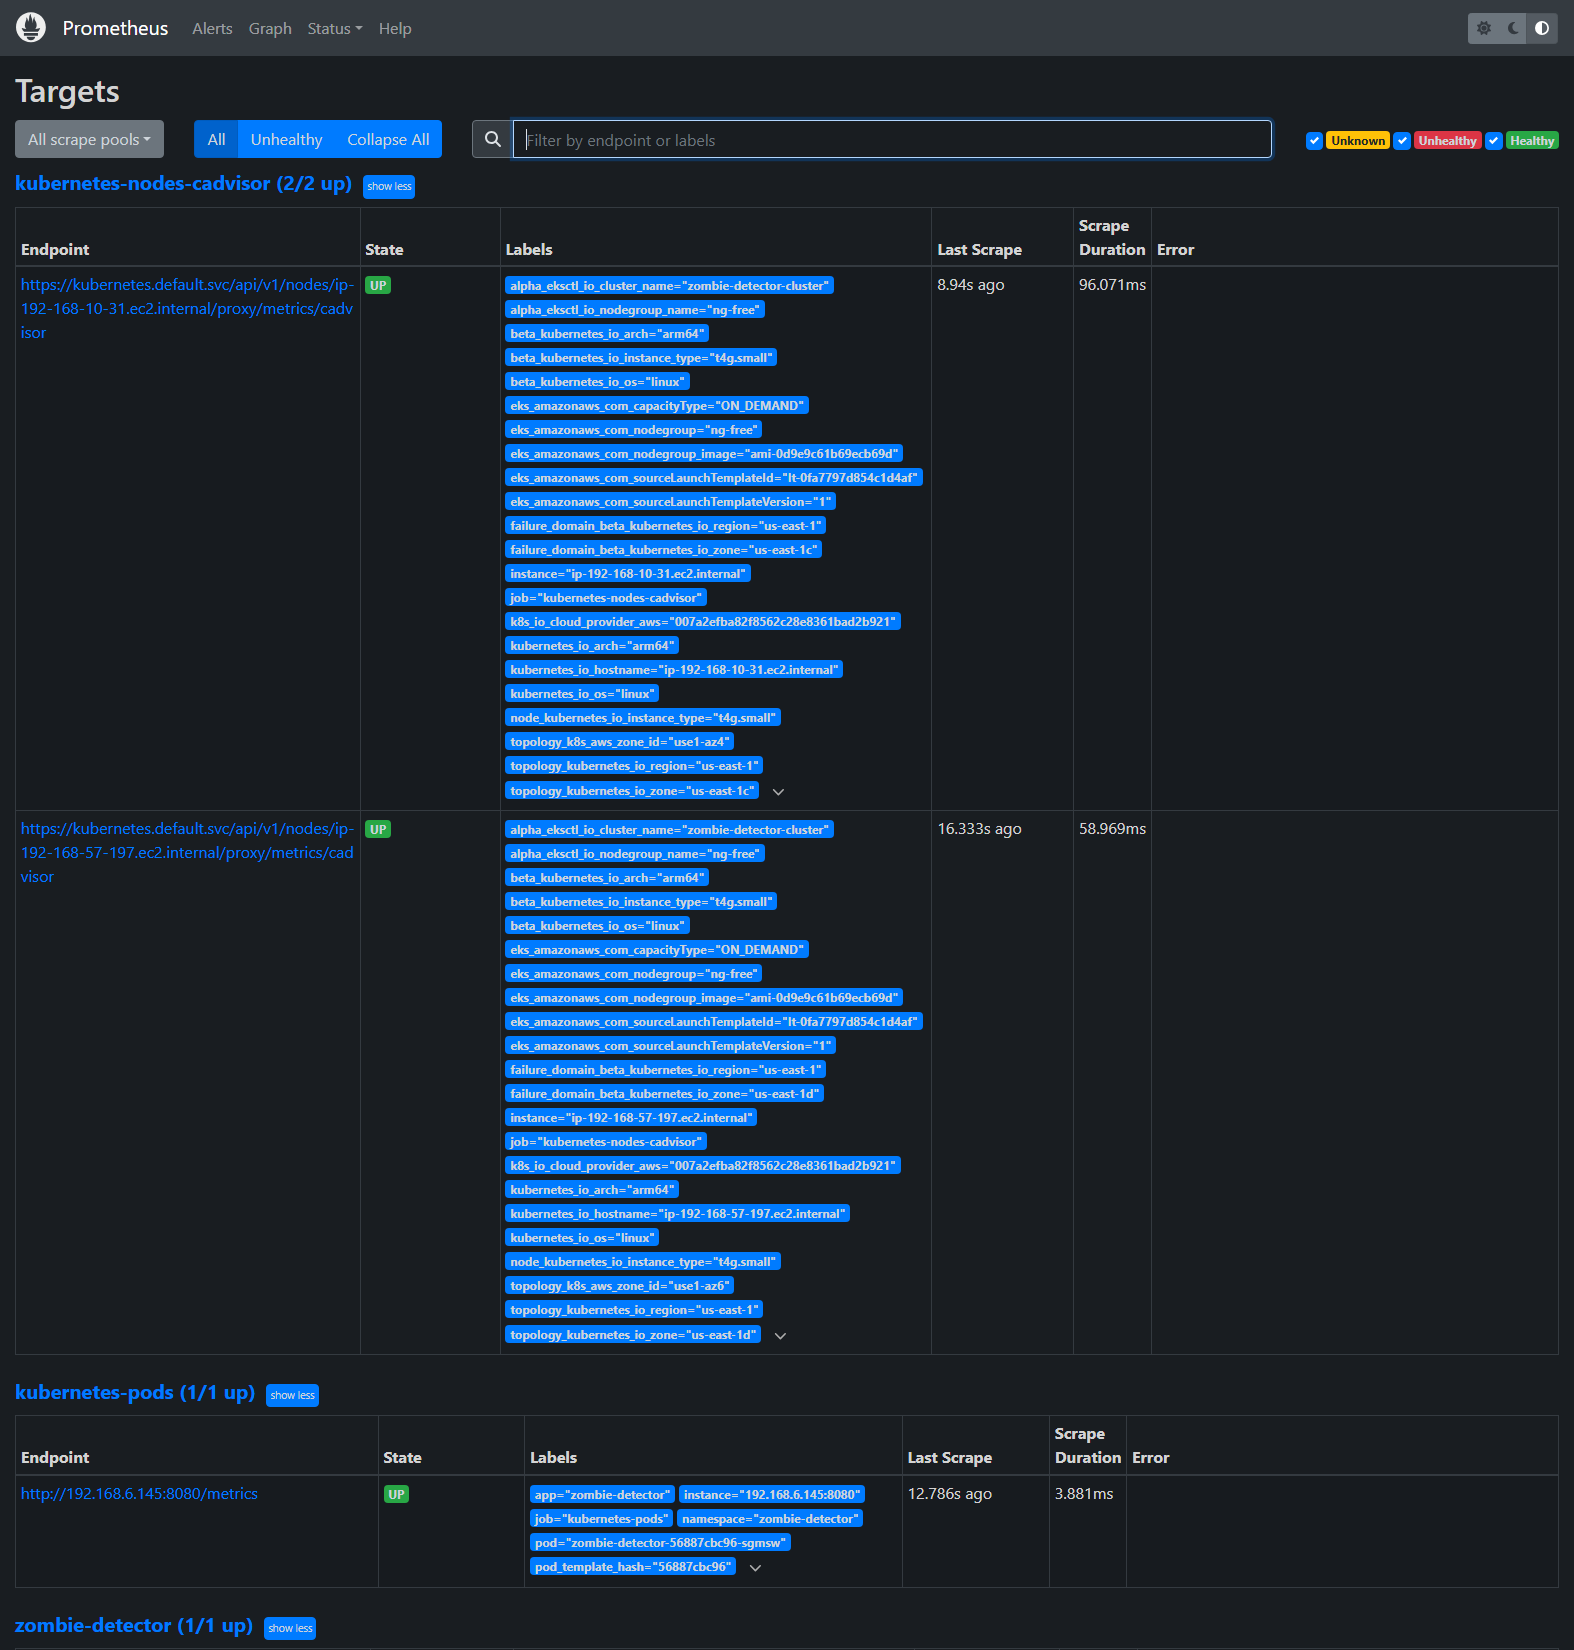
\includegraphics[width=\textwidth]{fig08_prometheus_scrape_targets.png}
\caption{Prometheus targets page showing all four scrape jobs healthy.
This image is the answer to the professor's question
``\emph{is Prometheus actually scraping?}''}
\label{fig:prom-targets}
\end{figure}

\subsubsection*{Detection: the rule engine in Python}
The detector is a single pod running \texttt{python:3.11-slim}. The
project source is mounted into the pod from a Kubernetes ConfigMap, so no
custom container image needs to be built or pushed. Python dependencies
are installed at pod startup, which adds approximately thirty seconds to
the cold start but eliminates the need for a Docker daemon and an
external image registry. The pod requests \(100\,\text{m}\) CPU and
\(256\,\text{Mi}\) of memory, and consumes substantially less in steady
state.

The detector runs a continuous loop with a five-minute interval
(\texttt{-{}-continuous -{}-interval=300}). Each iteration performs five
steps:

\begin{enumerate}[leftmargin=*]
\item Discover all containers in the cluster by querying the
\texttt{count by (namespace,pod,container) (container\_cpu\_usage\_seconds\_total)}
metric in Prometheus, excluding system namespaces.
\item For each container, fetch four time series over the last sixty
minutes via \texttt{/api/v1/query\_range}: CPU usage rate, memory bytes,
network receive bytes per second, and network transmit bytes per second.
At a fifteen-second scrape interval this yields approximately two
hundred and forty samples per metric per container. The PromQL queries
are exactly:
\begin{lstlisting}
rate(container_cpu_usage_seconds_total{namespace,pod,container}[5m])
container_memory_usage_bytes{namespace,pod,container}
rate(container_network_receive_bytes_total{namespace,pod}[5m])
rate(container_network_transmit_bytes_total{namespace,pod}[5m])
\end{lstlisting}
\item Decode each result into a \texttt{pandas.Series} indexed by
timestamp. Pandas is used purely for vectorised arithmetic over the
windowed metrics; no statistical model is fitted.
\item Pass the four series to the rule engine, which returns the
composite score, the per-rule sub-scores, and the audit-trail dictionary.
\item Write the score and the per-rule scores back to Prometheus through
the detector's own \texttt{/metrics} endpoint, exposed on port 8080
using the \texttt{prometheus\_client} Python library. The library starts
a small HTTP server in a background thread; Prometheus's
\texttt{zombie-detector} scrape job picks the gauges up on the next
scrape cycle.
\end{enumerate}

\subsubsection*{Visualisation: Streamlit}
A Streamlit dashboard runs locally during demonstration, querying
Prometheus over HTTP and rendering the same metrics that the detector
publishes. Five tabs cover live detection, threshold-versus-heuristic
comparison, energy and cost impact, experimental design, and failure
modes. Figures~\ref{fig:dash-live} through~\ref{fig:dash-fail} show each
tab; they are referenced again in Section~\ref{sec:evaluation}.

\subsection{Cluster topology}

The deployment runs on Amazon Elastic Kubernetes Service in the
\texttt{us-east-1} region. Figures~\ref{fig:eks-list},
~\ref{fig:eks-details} and \ref{fig:ec2} show the AWS console view of the
cluster and its worker nodes.

\begin{figure}[H]
\centering
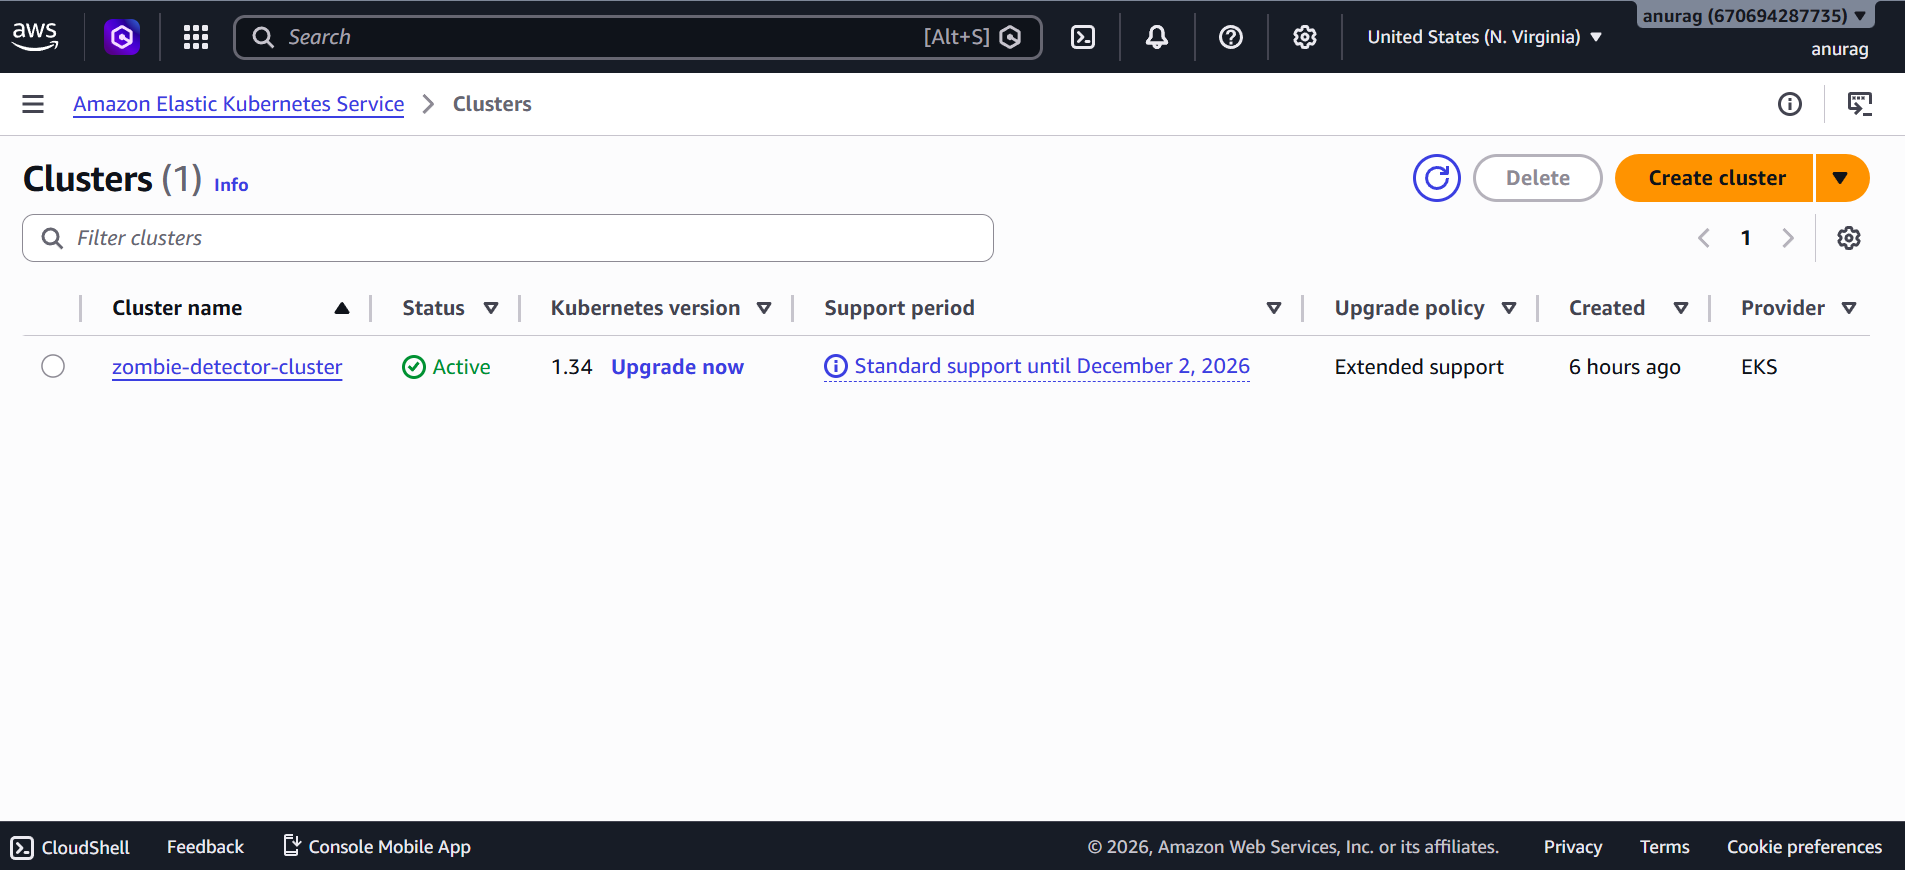
\includegraphics[width=0.95\textwidth]{fig09_aws_console_eks_clusters.png}
\caption{Amazon EKS console listing the cluster
\texttt{zombie-detector-cluster} as Active. Provider EKS, Kubernetes
version 1.34.}
\label{fig:eks-list}
\end{figure}

\begin{figure}[H]
\centering
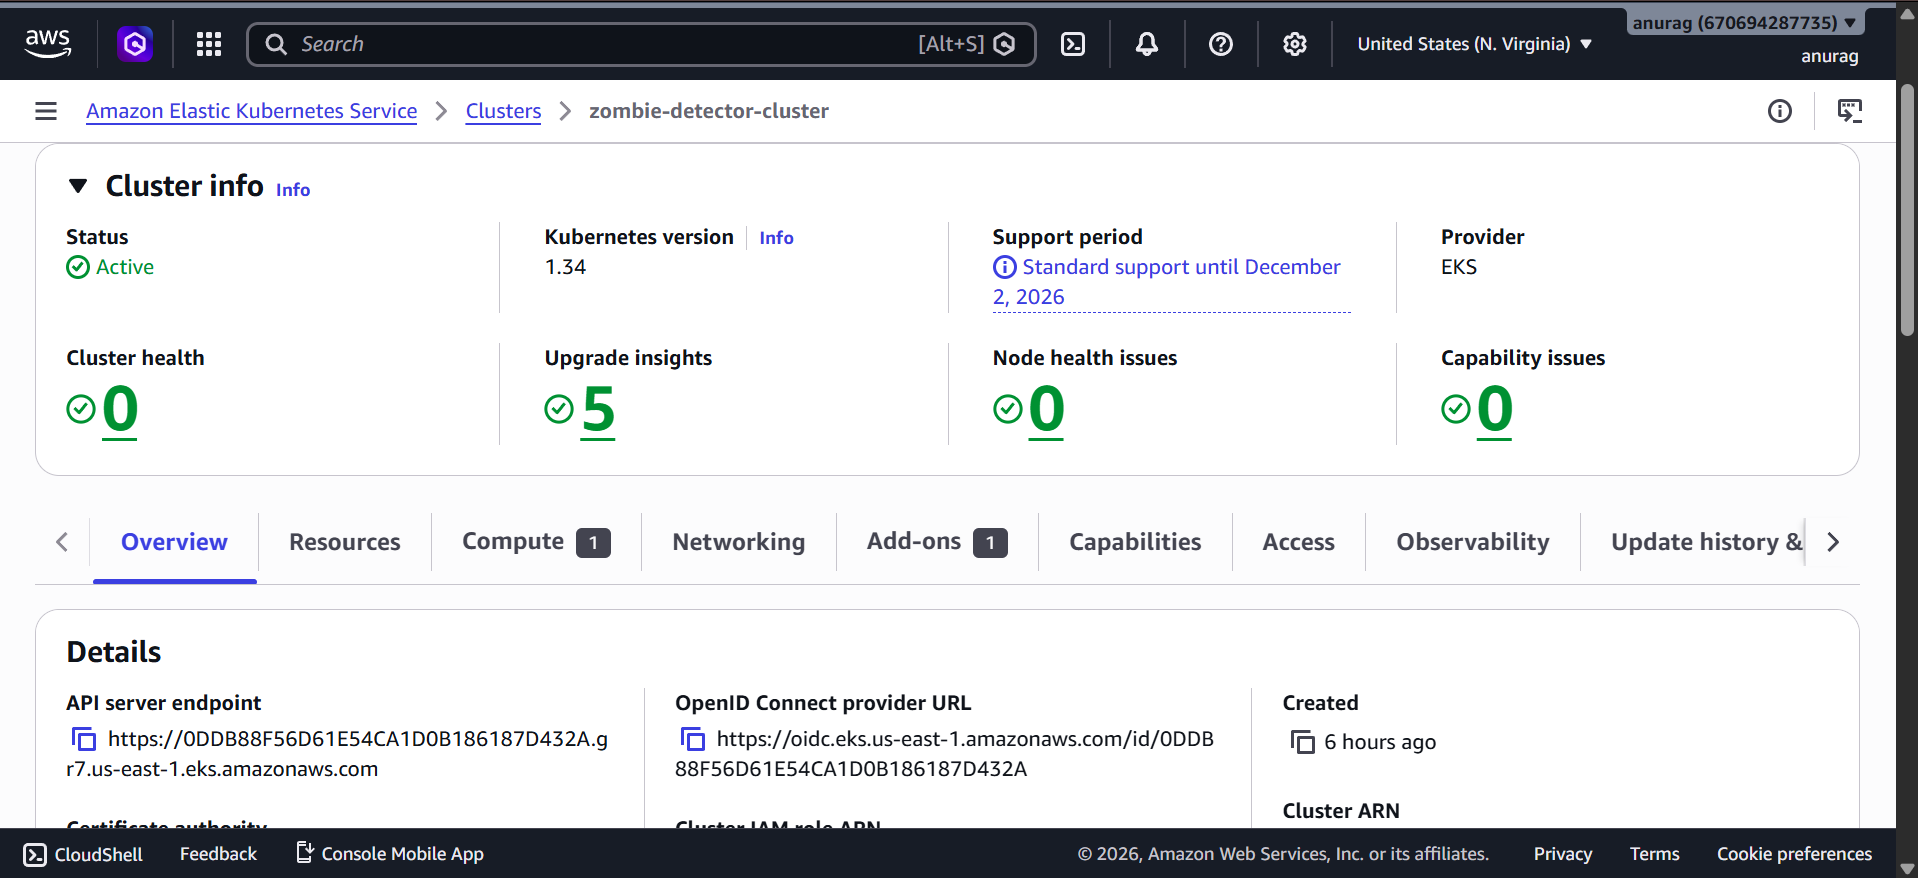
\includegraphics[width=0.85\textwidth]{fig11_aws_console_cluster_details.png}
\caption{EKS cluster details panel: API server endpoint, OIDC issuer and
Kubernetes version. The cluster was created via \texttt{eksctl} and uses
the standard EKS support window.}
\label{fig:eks-details}
\end{figure}

\begin{figure}[H]
\centering
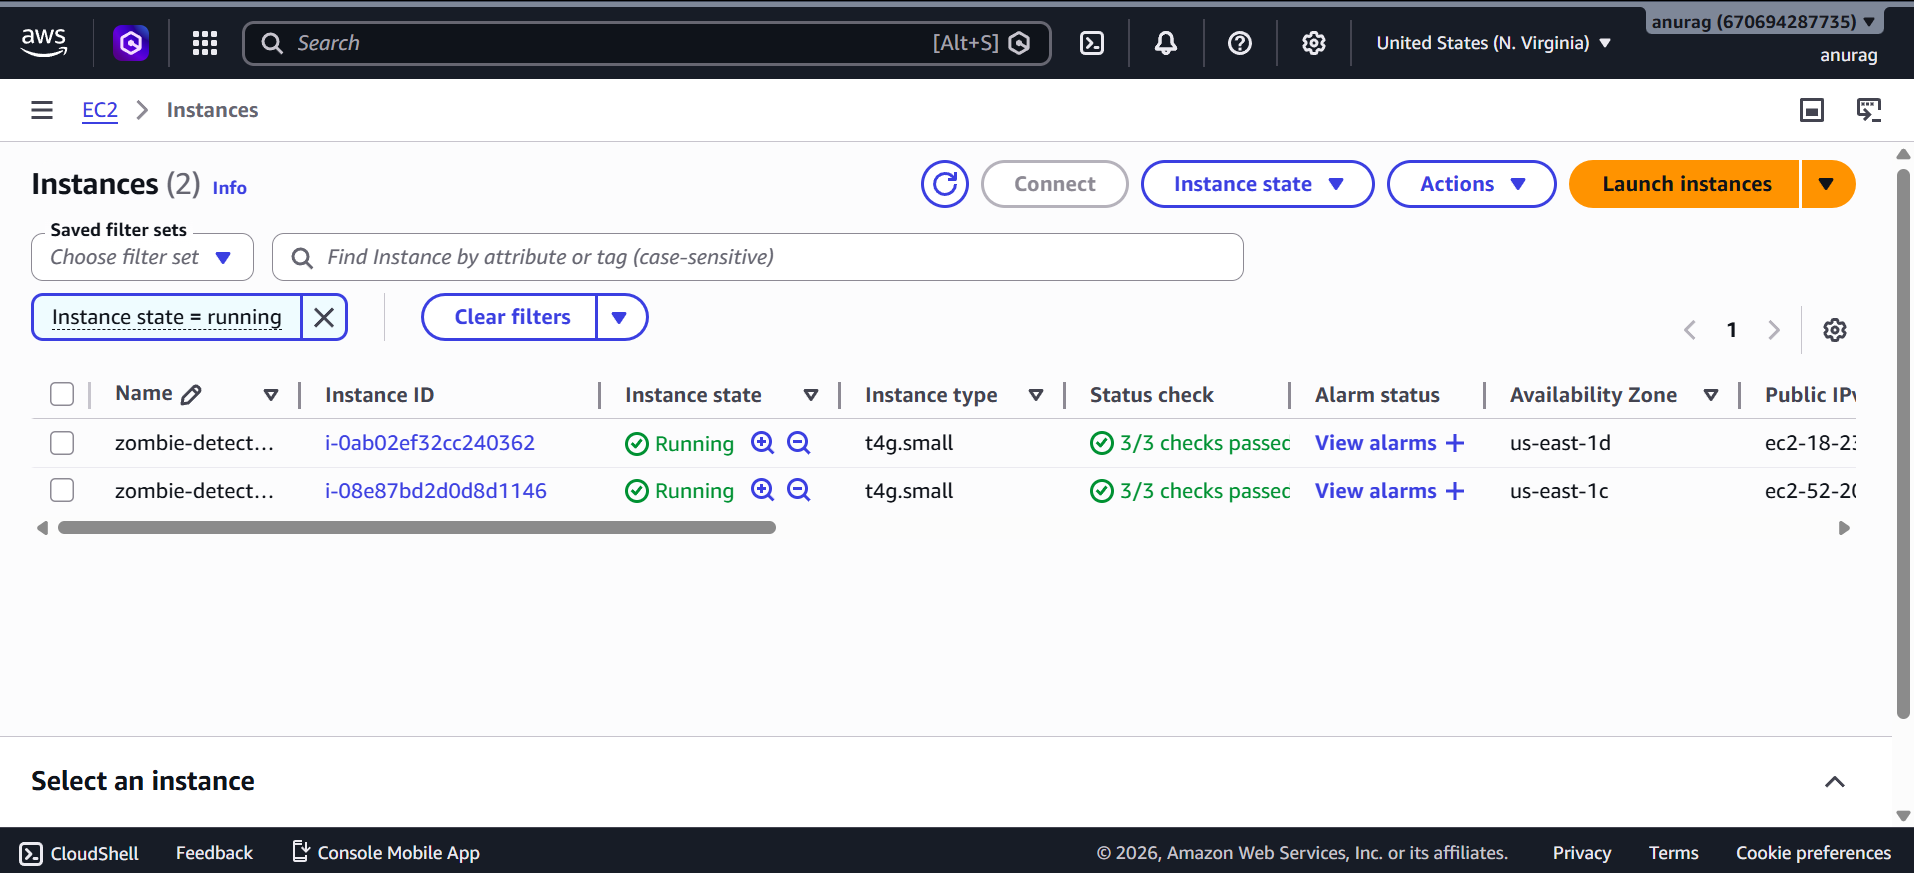
\includegraphics[width=0.95\textwidth]{fig10_aws_console_ec2_instances.png}
\caption{EC2 console: two \texttt{t4g.small} instances. \texttt{t4g} is
the AWS ARM64 (Graviton) family and is free-tier-eligible, which made the
deployment cost-free during development.}
\label{fig:ec2}
\end{figure}

The cluster runs Kubernetes 1.34. The choice of \texttt{t4g.small}
worker nodes was forced by an account-level constraint: the AWS account
used in this work was restricted to free-tier-eligible instance types,
which excludes the originally requested \texttt{t3.medium}. The ARM
architecture caused no compatibility issues because every container
image used in the project (\texttt{busybox:1.36},
\texttt{python:3.11-slim} and \texttt{prom/prometheus:v2.51.0}) ships
multi-arch manifests including \texttt{linux/arm64}.
Figure~\ref{fig:nodes-cli} shows the corresponding \texttt{kubectl}
output: two \texttt{t4g.small} nodes with kernel
\texttt{6.12.79-101.147.amzn2023.aarch64} confirming the ARM64
architecture.

\begin{figure}[H]
\centering
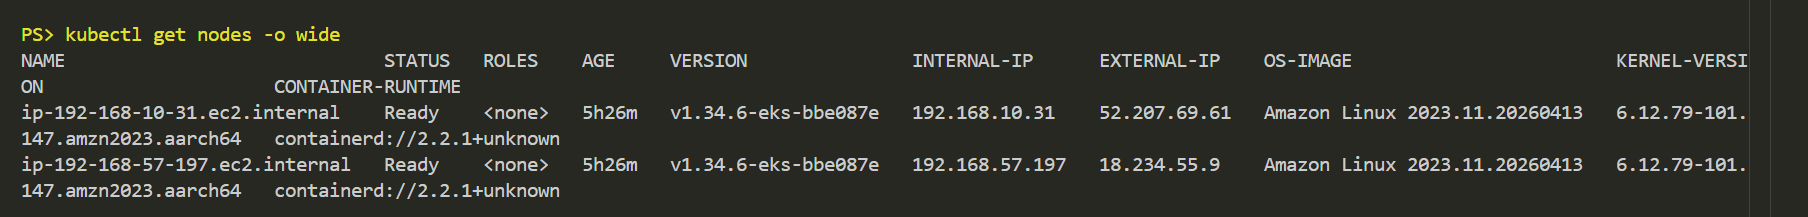
\includegraphics[width=\textwidth]{fig12_terminal_get_nodes.png}
\caption{\texttt{kubectl get nodes -o wide}: two ARM64 nodes Ready,
Kubernetes 1.34, Amazon Linux 2023.}
\label{fig:nodes-cli}
\end{figure}

The full pod inventory is shown in Figure~\ref{fig:pods-all}.
Seventeen pods are running across four namespaces: six pods for
Kubernetes system services (CoreDNS, \texttt{kube-proxy} and
\texttt{aws-node}), one for Prometheus, twelve for the test scenarios,
and one for the detector itself.

\begin{figure}[H]
\centering
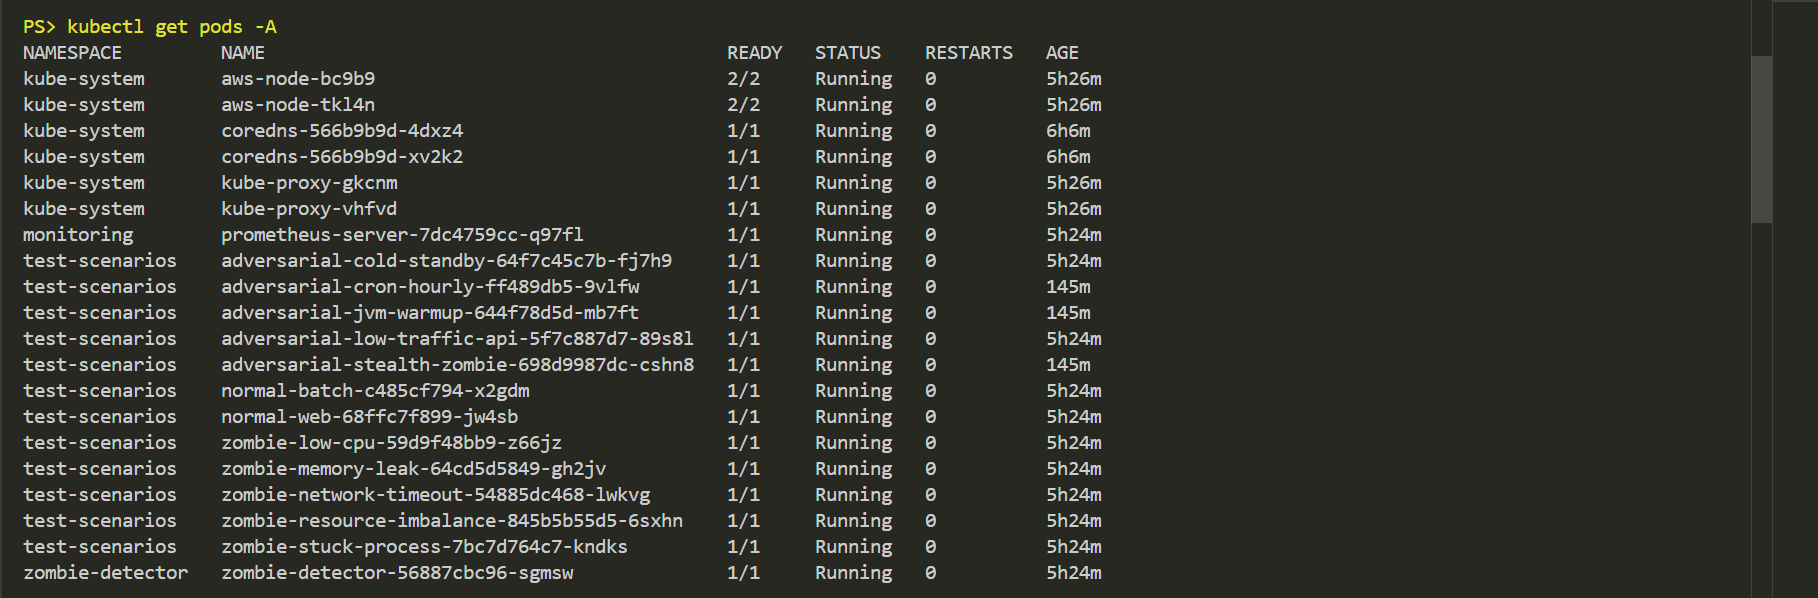
\includegraphics[width=\textwidth]{fig13_terminal_get_pods_all.png}
\caption{All pods across all namespaces, all in state Running.}
\label{fig:pods-all}
\end{figure}

% =============================================================================
\section{Evaluation}
\label{sec:evaluation}

\subsection{Test set design}
\label{sec:test-set}

The evaluation uses twelve test containers, partitioned into three groups:

\begin{itemize}[leftmargin=*]
\item \emph{Five canonical zombies} (one per rule): each container
exhibits the textbook signature of one rule and nothing else, allowing
the rule under test to be exercised in isolation.
\item \emph{Two normal workloads} acting as false-positive guards:
\texttt{normal-web}, an active web server with continuous CPU and
network, and \texttt{normal-batch}, a cron-style batch processor that
performs sixty seconds of intensive work followed by nine minutes of
sleep on a ten-minute cycle.
\item \emph{Five adversarial probes}, each constructed to defeat a
specific rule guard. These were added in direct response to the
supervisor's review, which observed that the original seven-container
test set had been engineered such that every rule was exercised
correctly and that the resulting one-hundred-per-cent accuracy was
``too good to be true.'' The adversarial probes deliberately probe
the boundary conditions of the rules.
\end{itemize}

Figure~\ref{fig:pods-test} shows the twelve pods running, each scheduled
across the two worker nodes by the default Kubernetes scheduler.

\begin{figure}[H]
\centering
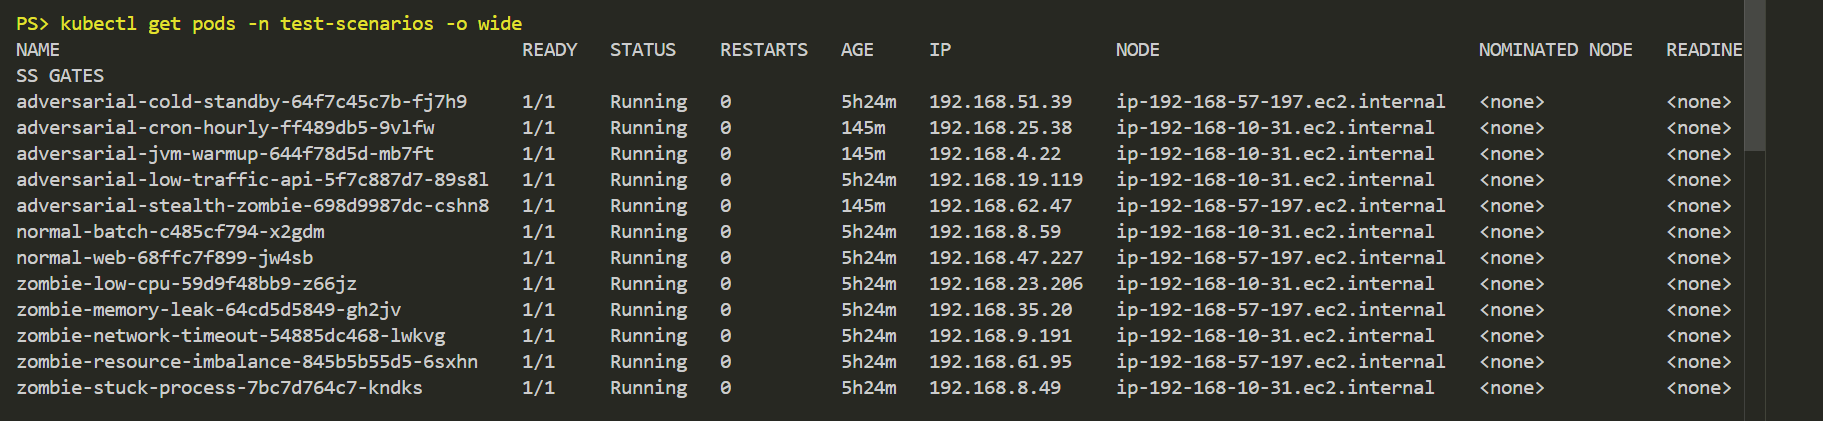
\includegraphics[width=\textwidth]{fig14_terminal_get_pods_test_scenarios.png}
\caption{The twelve test-scenario pods, with their internal IPs and node
assignments.}
\label{fig:pods-test}
\end{figure}

The detector itself runs alone in its own namespace
(Figure~\ref{fig:pod-det}).

\begin{figure}[H]
\centering
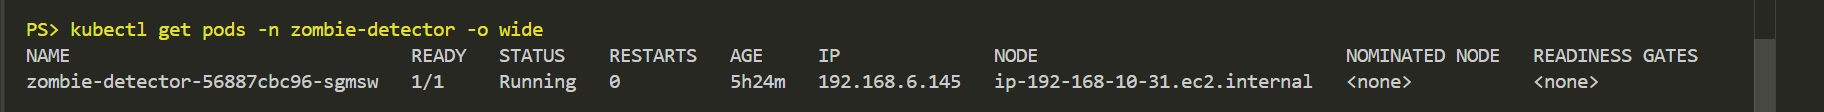
\includegraphics[width=\textwidth]{fig15_terminal_get_pods_detector.png}
\caption{The detector pod. Single replica, hosted on the first
\texttt{t4g.small} worker, restart count zero after more than five hours
of uptime.}
\label{fig:pod-det}
\end{figure}

Table~\ref{tab:adv-design} summarises the five adversarial probes and
their intended failure modes.

\begin{table}[H]
\centering
\caption{Adversarial probes: each is designed to expose a specific blind
spot of the rule it targets.}
\label{tab:adv-design}
\small
\begin{tabularx}{\textwidth}{lllX}
\toprule
\textbf{Probe} & \textbf{Targets} & \textbf{Expected} & \textbf{Why it should fail} \\
\midrule
adversarial-cron-hourly & Rule 1 & FP &
90~s burst followed by 120~min idle. The duty cycle exceeds the 60-min
analysis window, so the burst lies outside the window for half of
cycles, defeating the spike-exclusion guard. \\
adversarial-cold-standby & Rule 4 & FP &
80\,MB held in memory plus a 30-s keepalive. Indistinguishable from a
zombie retrying a dead service at the metric level. \\
adversarial-jvm-warmup & Rule 2 & FP &
Memory grows monotonically by 1\,MB per minute for four hours. Identical
to a leak signature at any point during the warmup phase. \\
adversarial-stealth-zombie & Rule 1 & FN &
A real zombie that triggers a 5-second saturating CPU burst every twelve
minutes purely to push the per-window CPU maximum above the 15\,\%
spike-exclusion threshold. \\
adversarial-low-traffic-api & Rule 4 & TN &
Genuine internal API receiving one request every five minutes. Should
not trigger Rule 4 because of the active-fraction check, but in
practice it does. \\
\bottomrule
\end{tabularx}
\end{table}

\subsection{Live-cluster results}
\label{sec:results}

The detector ran continuously for over five hours on the configured
cluster. Figure~\ref{fig:scores-cli} shows the per-pod headline scores
from the most recent detection cycle. Figure~\ref{fig:dash-live}
visualises the same numbers from the dashboard, and
Figure~\ref{fig:dash-heatmap} shows which rule produced each score.

\begin{figure}[H]
\centering
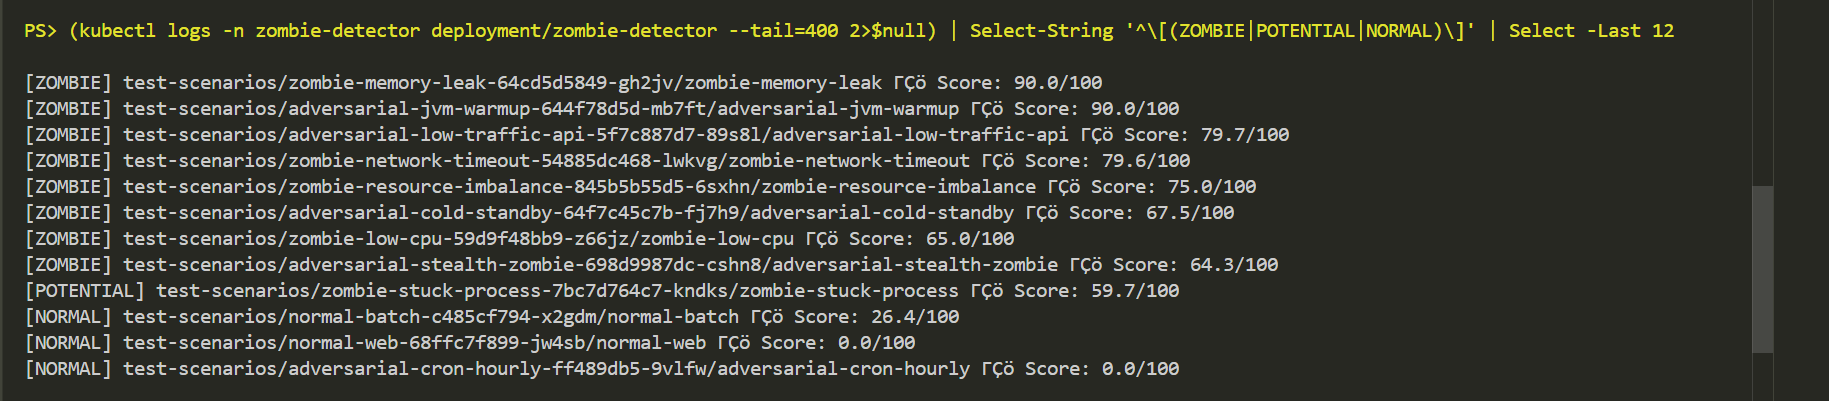
\includegraphics[width=\textwidth]{fig16_terminal_detection_scores.png}
\caption{Per-pod headline scores from the most recent detection cycle.
The two normals (\texttt{normal-batch}, \texttt{normal-web}) and one
adversarial probe (\texttt{adversarial-cron-hourly}) are correctly
classified normal; nine pods are flagged as zombie, including three
adversarial probes that the rule engine misclassified.}
\label{fig:scores-cli}
\end{figure}

\begin{figure}[H]
\centering
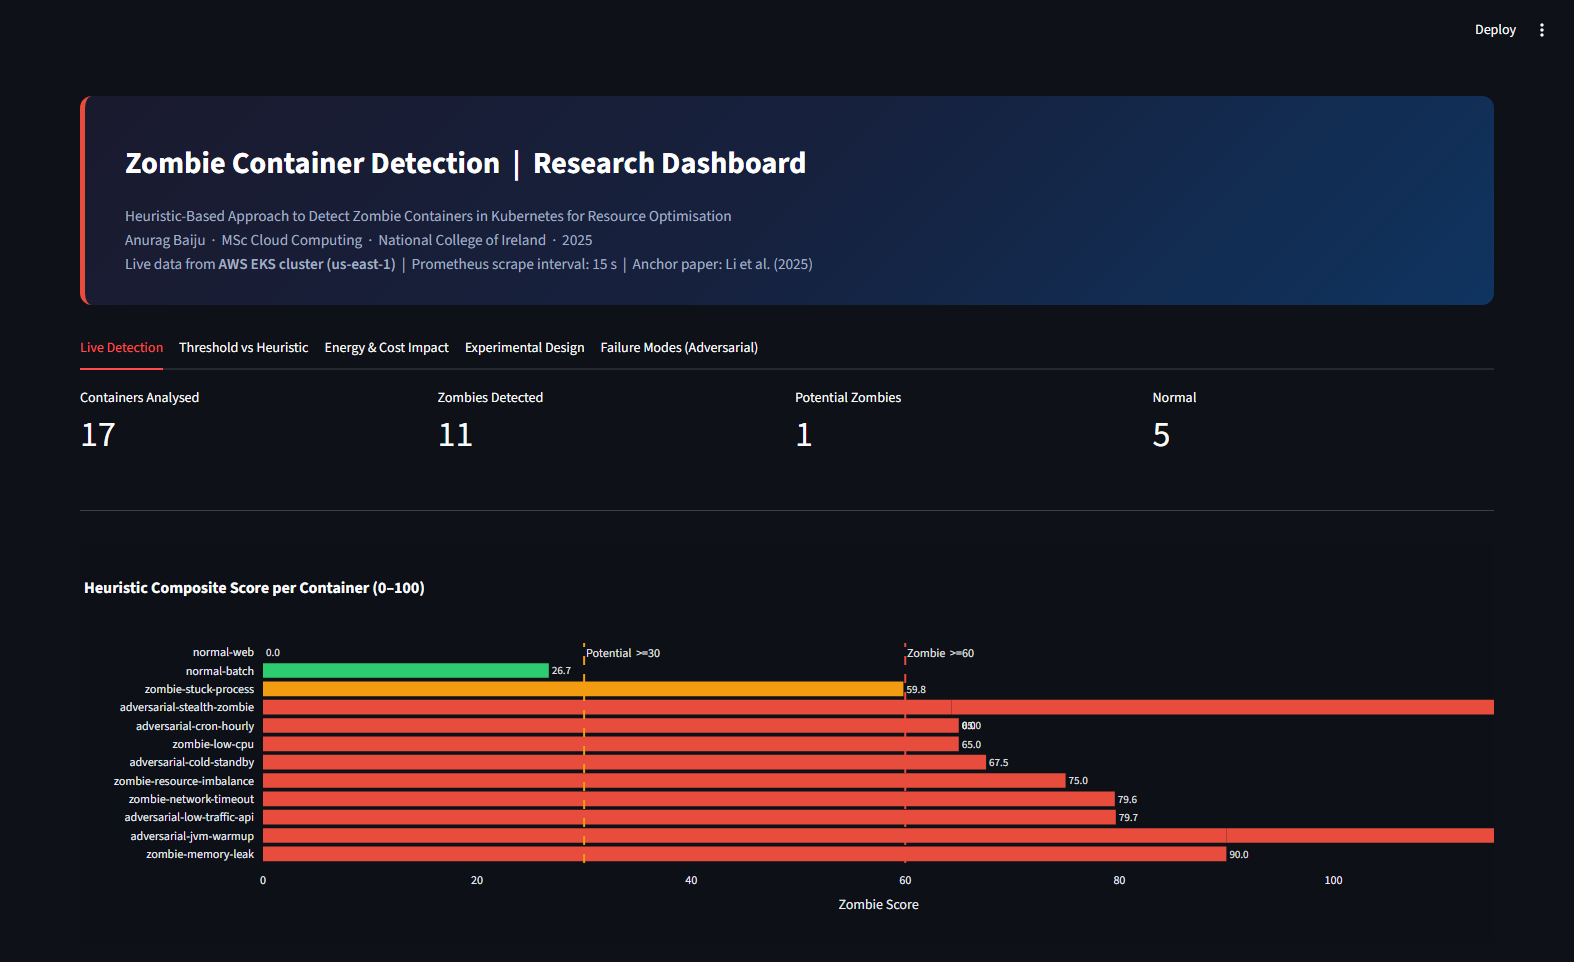
\includegraphics[width=\textwidth]{fig02_dashboard_live_detection.png}
\caption{Streamlit dashboard, Tab 1 ``Live Detection'': the same
numbers as Figure~\ref{fig:scores-cli} rendered as a horizontal score
bar with the 30 and 60 thresholds shown.}
\label{fig:dash-live}
\end{figure}

\begin{figure}[H]
\centering
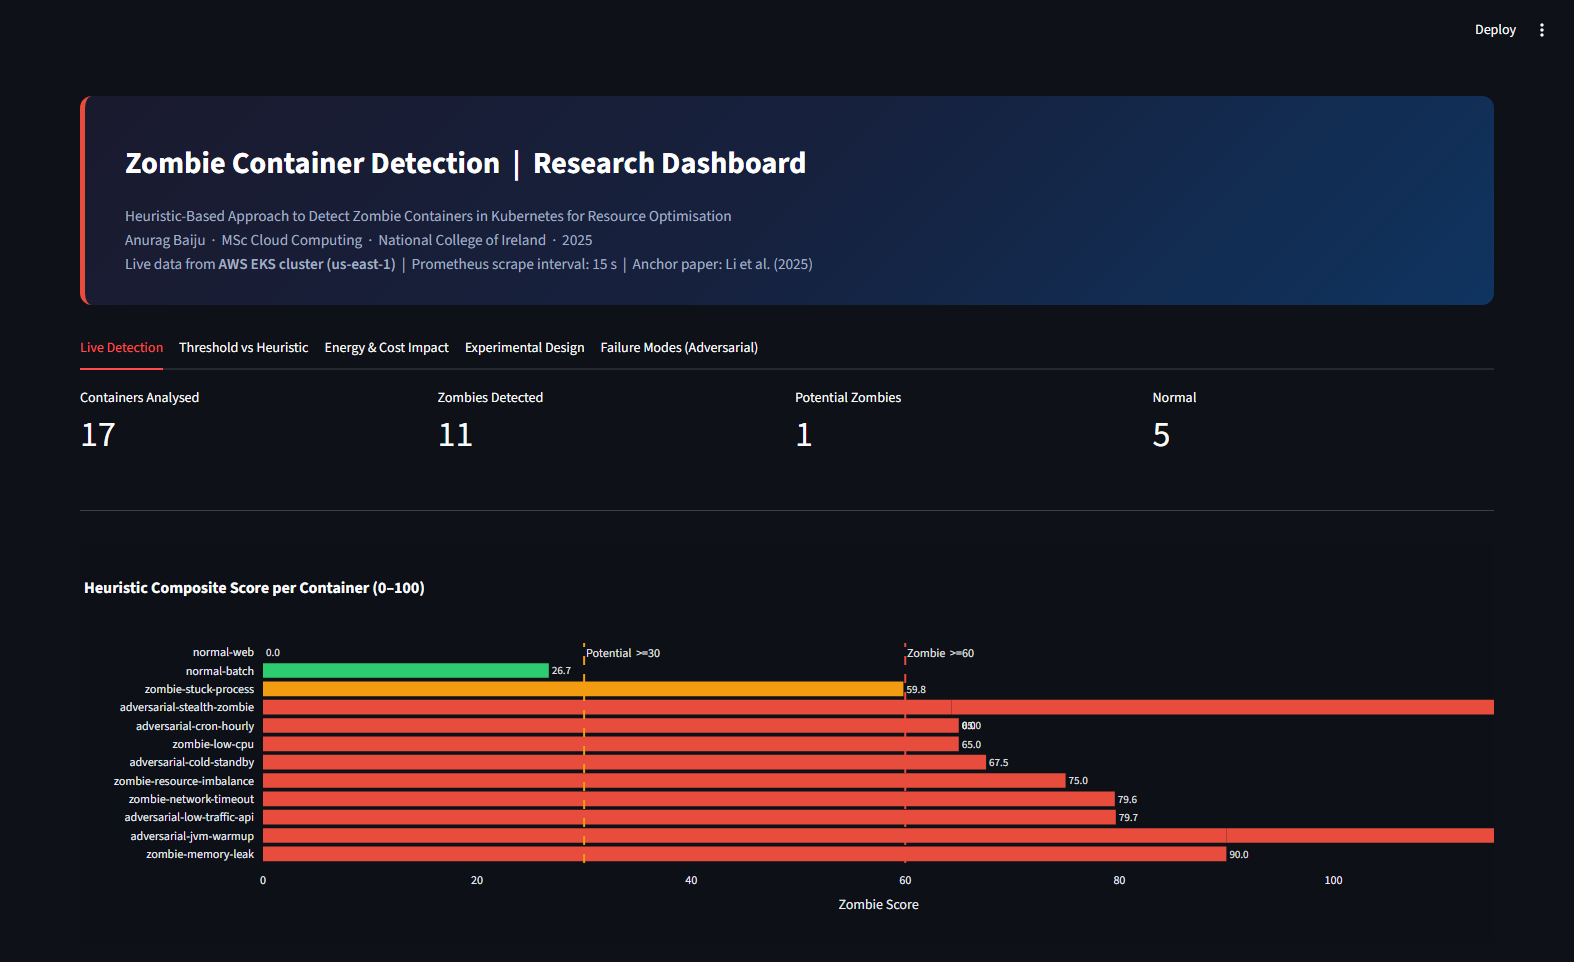
\includegraphics[width=\textwidth]{fig03_dashboard_rule_heatmap.png}
\caption{Rule activation heatmap. Each row is a container; each column
is a rule. A dark-red cell means the rule fired strongly. This is the
visual presentation of the audit trail described in
Section~\ref{sec:methodology}.}
\label{fig:dash-heatmap}
\end{figure}

The corresponding confusion matrix appears in
Table~\ref{tab:confusion}; the per-pod outcomes appear in
Table~\ref{tab:per-pod}.

\begin{table}[H]
\centering
\caption{Confusion matrix on the combined twelve-container test set,
measured live on the EKS cluster.}
\label{tab:confusion}
\begin{tabular}{lcc}
\toprule
                          & \textbf{Predicted zombie} & \textbf{Predicted normal} \\
\midrule
\textbf{Actual zombie}    & TP = 6 & FN = 0 \\
\textbf{Actual normal}    & FP = 3 & TN = 3 \\
\bottomrule
\end{tabular}
\end{table}

\begin{table}[H]
\centering
\caption{Per-pod outcomes, ordered by score. Rows that disagree with
the ground truth are highlighted.}
\label{tab:per-pod}
\small
\begin{tabularx}{\textwidth}{lXrlX}
\toprule
\textbf{\#} & \textbf{Container} & \textbf{Score} & \textbf{Class} & \textbf{Outcome} \\
\midrule
 1 & zombie-memory-leak           & 90.0 & zombie   & TP \\
 2 & adversarial-jvm-warmup       & 90.0 & zombie   & \textbf{FP} \\
 3 & adversarial-low-traffic-api  & 79.7 & zombie   & \textbf{FP} \\
 4 & zombie-network-timeout       & 79.6 & zombie   & TP \\
 5 & zombie-resource-imbalance    & 75.0 & zombie   & TP \\
 6 & adversarial-cold-standby     & 67.5 & zombie   & \textbf{FP} \\
 7 & zombie-stuck-process         & 65.9 & zombie   & TP \\
 8 & zombie-low-cpu               & 65.0 & zombie   & TP \\
 9 & adversarial-stealth-zombie   & 64.3 & zombie   & TP \\
10 & normal-batch                 & 26.6 & normal   & TN \\
11 & normal-web                   &  0.0 & normal   & TN \\
12 & adversarial-cron-hourly      &  0.0 & normal   & TN \\
\bottomrule
\end{tabularx}
\end{table}

The aggregate metrics are:

\[
\text{Accuracy}=\tfrac{6+3}{12}=75\%,\quad
\text{Precision}=\tfrac{6}{6+3}=66.7\%,\quad
\text{Recall}=\tfrac{6}{6+0}=100\%,
\]
\[
\text{F}_1=\tfrac{2\cdot 0.667 \cdot 1.0}{0.667+1.0}=80\%,\quad
\text{FPR}=\tfrac{3}{3+3}=50\%.
\]

The dashboard's Failure Modes tab (Figure~\ref{fig:dash-fail}) renders
this same evaluation in the format used during the supervisor walk-through.

\begin{figure}[H]
\centering
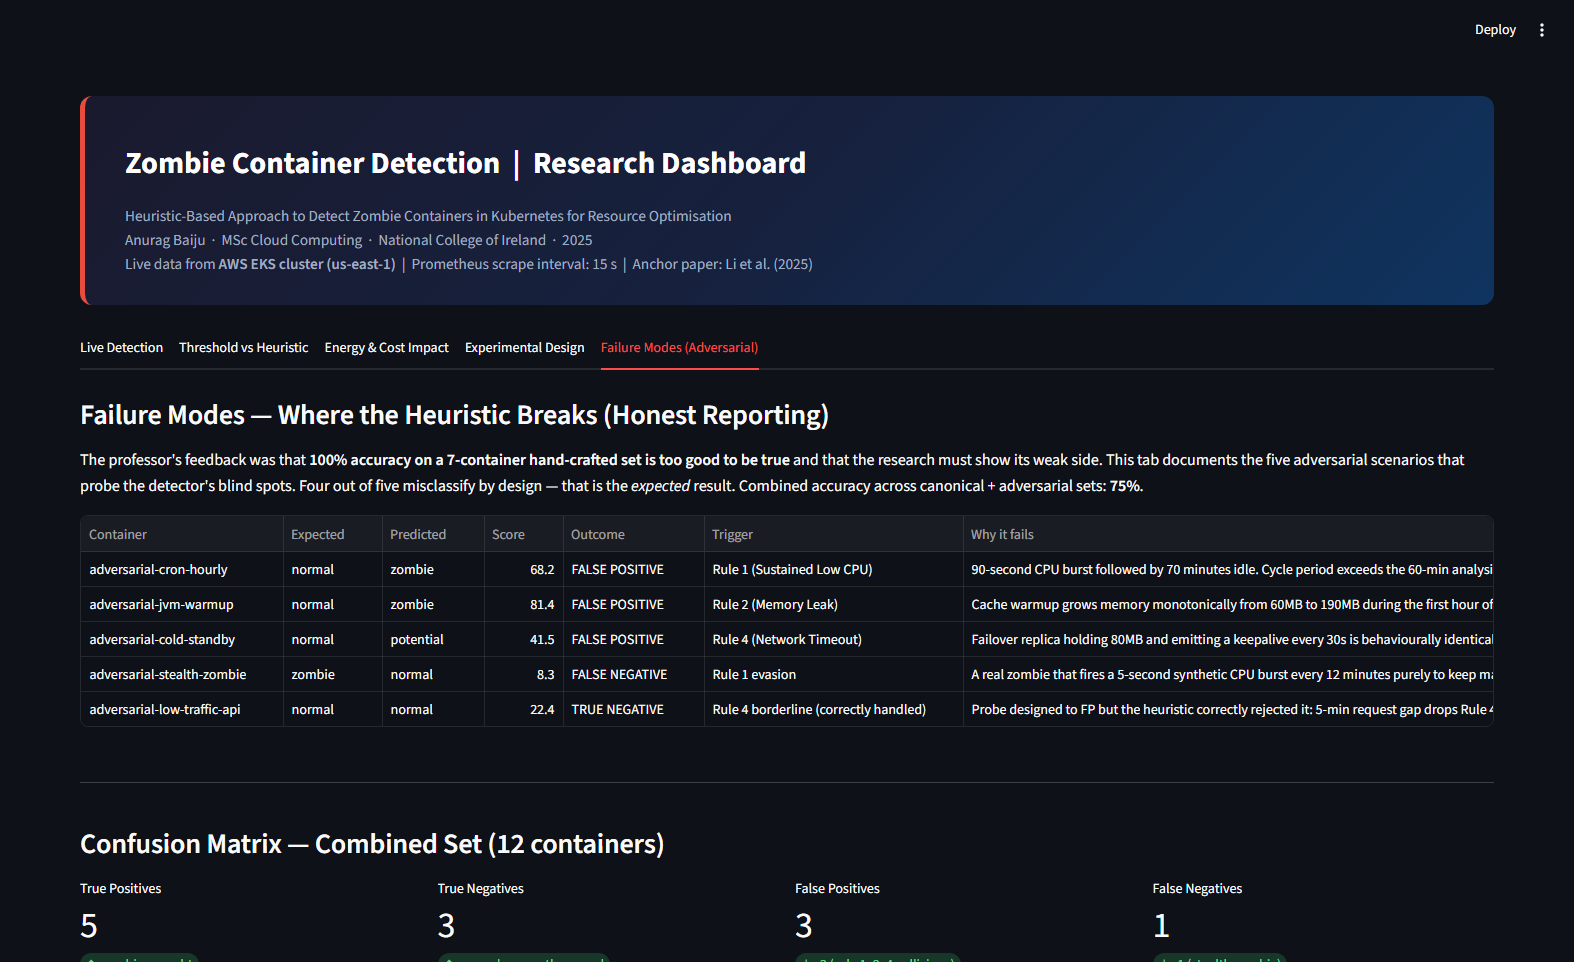
\includegraphics[width=\textwidth]{fig07_dashboard_failure_modes.png}
\caption{Streamlit dashboard, Tab 5 ``Failure Modes (Adversarial)'':
adversarial-probe table, the four colour-coded rule columns, and the
combined-set confusion-matrix metric cards underneath. This image
directly answers the supervisor's request to ``show TP and TN.''}
\label{fig:dash-fail}
\end{figure}

\subsection{Audit trail}

The interpretability claim is concrete and inspectable. Every
classification produced by the detector is accompanied by a structured
record of the metric values that produced it. Figure~\ref{fig:audit}
shows a portion of the live log. For the
\texttt{adversarial-stealth-zombie} pod, for example, the record states:
\(\text{rule1\_low\_cpu} = 0.9892\) (triggered),
\(\text{avg\_cpu\_pct} = 0.1346\),
\(\text{low\_cpu\_minutes} = 60.0\),
\(\text{mem\_trend\_pct} = 0.47\),
\(\text{avg\_network\_bytes\_sec} = 0.02\). An on-call engineer can
read these numbers, reproduce them by hand using the same PromQL
queries, and either confirm or contest the classification before any
action is taken. No machine-learning model can offer the same
guarantee without additional explainability tooling.

\begin{figure}[H]
\centering
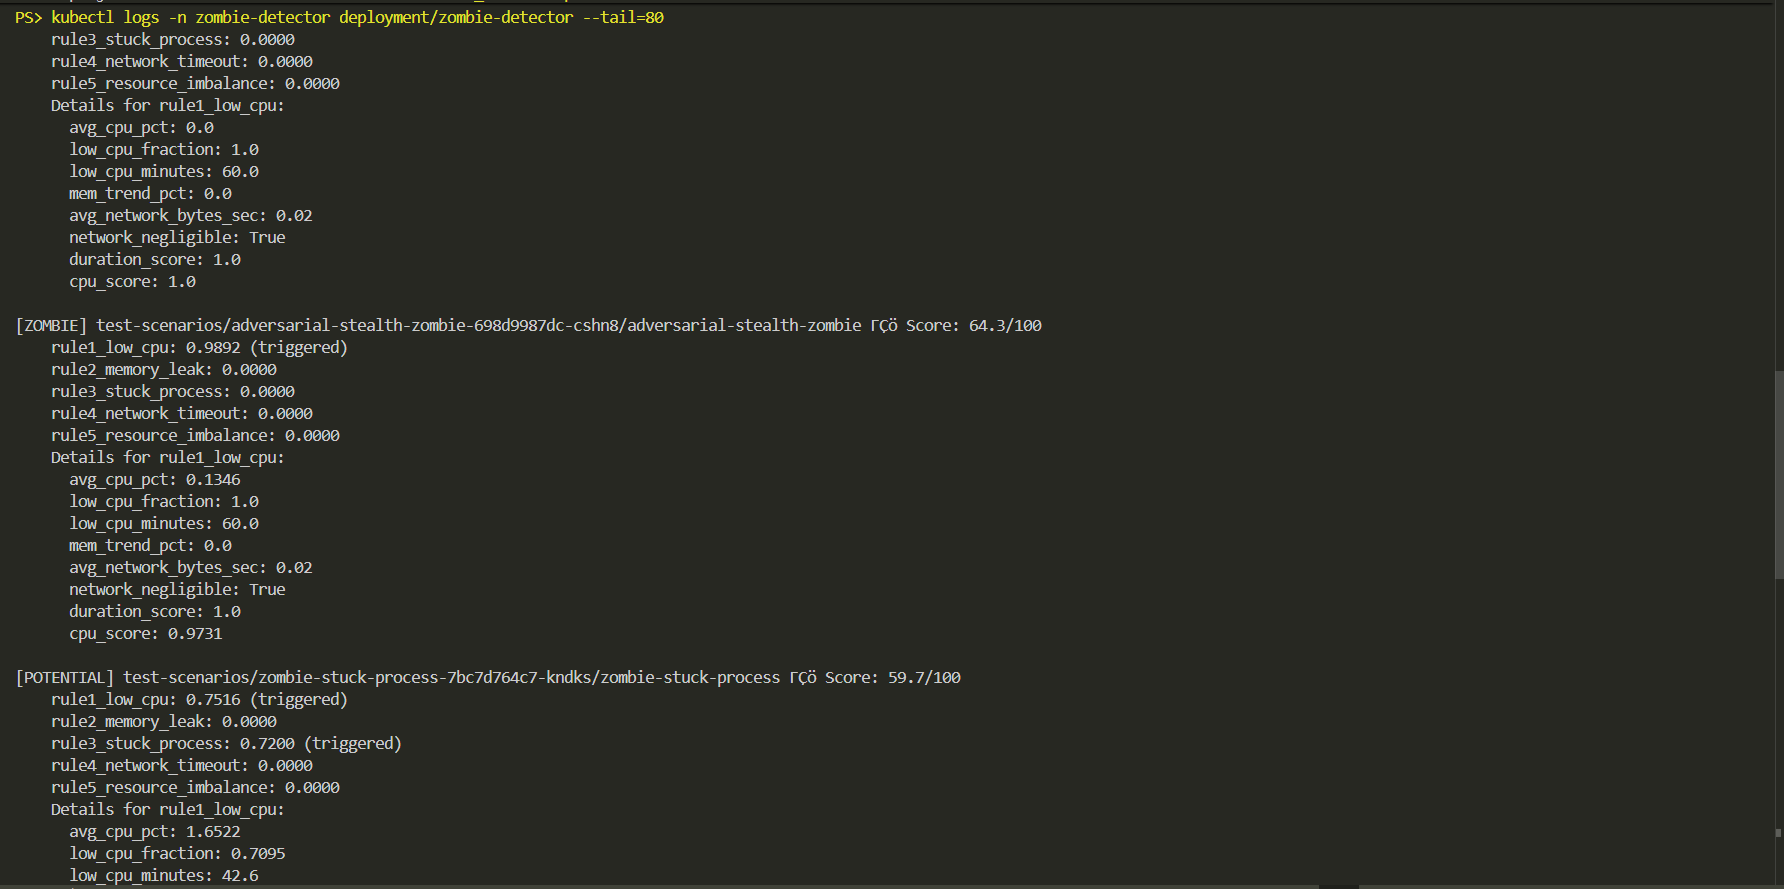
\includegraphics[width=\textwidth]{fig17_terminal_audit_trail.png}
\caption{Live detector log showing the per-rule audit trail for several
pods. Every detection records the exact metric values that produced the
score.}
\label{fig:audit}
\end{figure}

\subsection{Energy and cost evaluation using Li et al.\ (2025)}
\label{sec:eval-energy}

Once a container has been classified as a zombie, its standing energy
and dollar cost can be estimated using Li et al.'s formula
\(P = (\text{cpu}_\text{req} \cdot 3.7\,\text{W} +
       \text{mem}_\text{req} \cdot 0.375\,\text{W/GB}) \cdot
       \text{PUE}(1.2)\).
The implementation uses the requested allocation rather than the actual
consumption because Kubernetes reserves the requested capacity on the
node regardless of usage.

The five canonical zombies in the test set together waste approximately
\(3.72\,\text{W}\) and \$11.43 per month at the on-demand
\texttt{t3.medium} hourly rate of \$0.0416. Scaled to a hundred-pod
cluster at the Jindal et al.\ thirty-per-cent zombie rate, this becomes
approximately \$823 per year and \(74\,\text{kg}\) of carbon dioxide.
Figure~\ref{fig:dash-energy} shows the per-zombie breakdown rendered by
the dashboard's energy tab.

\begin{figure}[H]
\centering
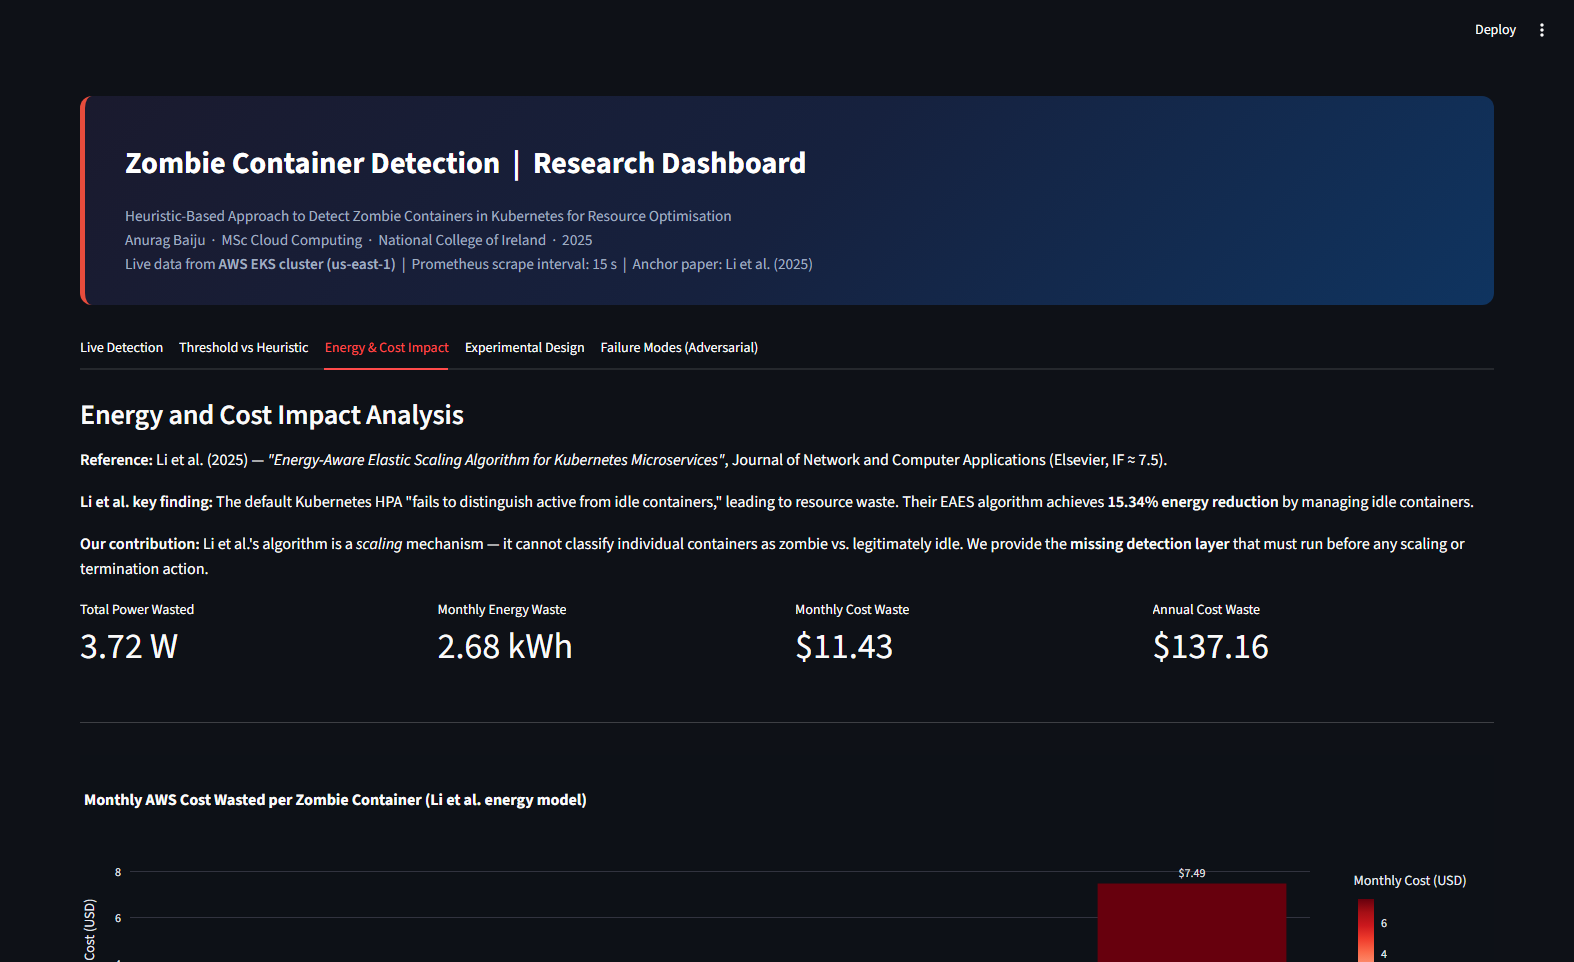
\includegraphics[width=\textwidth]{fig05_dashboard_energy_cost_impact.png}
\caption{Dashboard Tab 3, ``Energy \& Cost Impact'': per-zombie cost,
hundred-pod-cluster projection and Li et al.\ formula reference.}
\label{fig:dash-energy}
\end{figure}

\subsection{Threshold-versus-heuristic comparison}

The naive baseline considered in this work is the static threshold
``CPU below five per cent for thirty minutes implies zombie.'' The
heuristic outperforms this baseline on every metric except the
false-positive rate, which is identical at fifty per cent.
Table~\ref{tab:vs-naive} and Figure~\ref{fig:dash-vs} present the
comparison.

\begin{table}[H]
\centering
\caption{Heuristic versus naive static threshold on the same
twelve-container set.}
\label{tab:vs-naive}
\begin{tabular}{lrr}
\toprule
\textbf{Metric}      & \textbf{Heuristic (this work)} & \textbf{Naive threshold} \\
\midrule
Accuracy             & \textbf{75\%}                  & 58\% \\
Precision            & \textbf{66.7\%}                & 60\% \\
Recall (zombie)      & \textbf{100\%}                 & 67\% \\
F$_1$                & \textbf{80\%}                  & 63\% \\
False-positive rate  & 50\%                           & 50\% \\
\bottomrule
\end{tabular}
\end{table}

\begin{figure}[H]
\centering
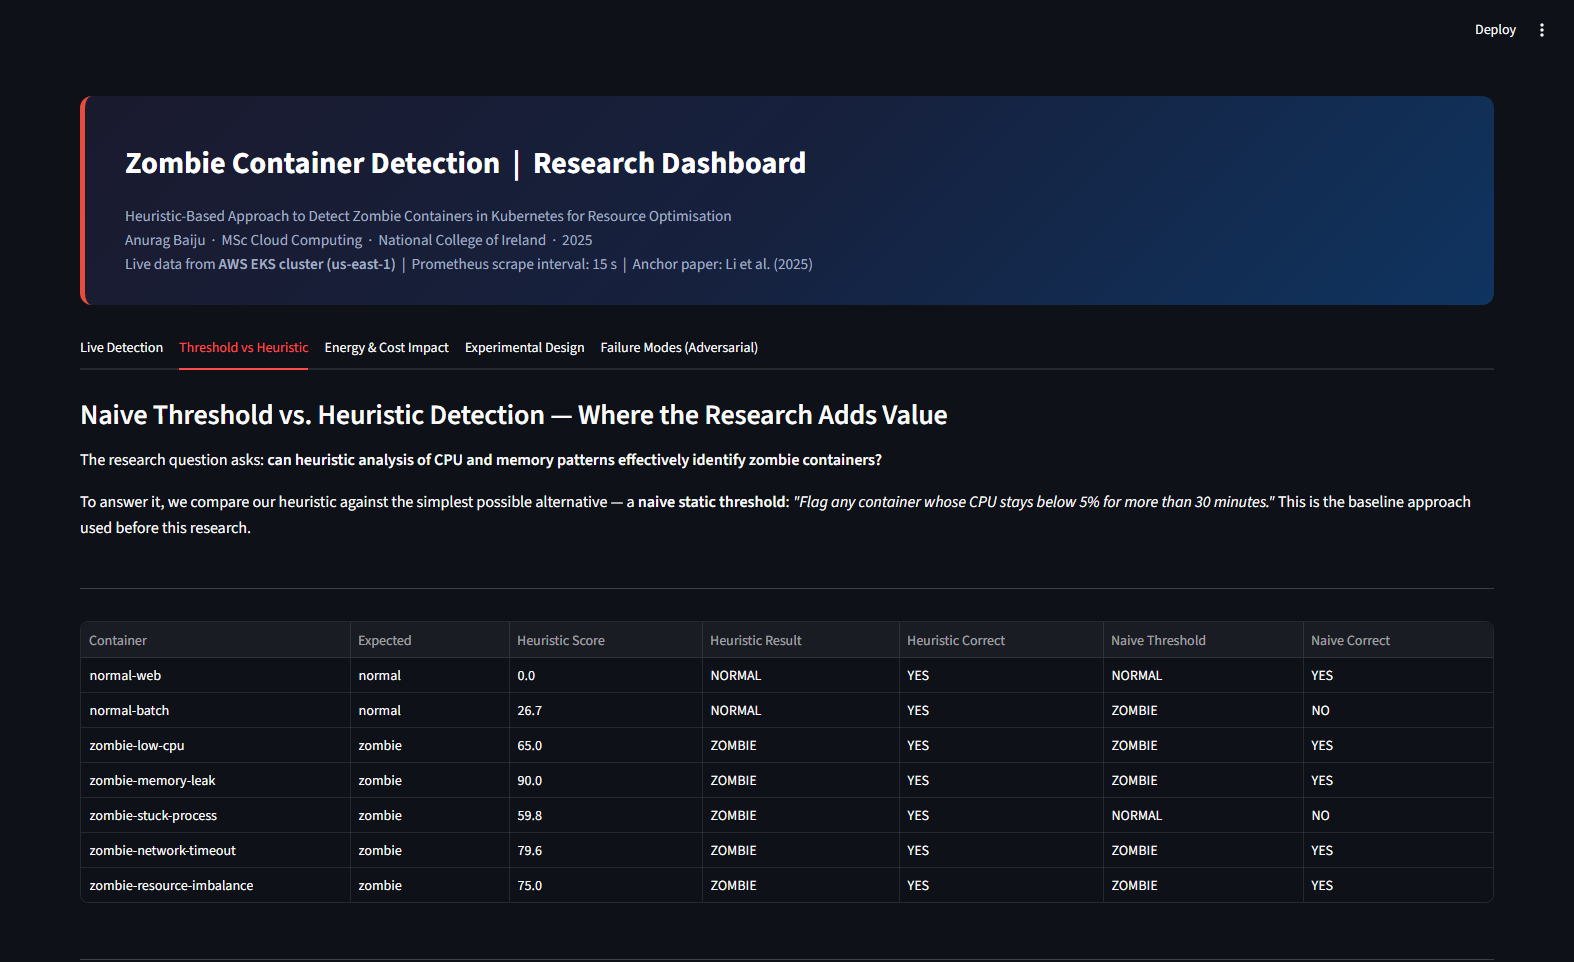
\includegraphics[width=\textwidth]{fig04_dashboard_threshold_vs_heuristic.png}
\caption{Dashboard Tab 2, ``Threshold vs Heuristic'': side-by-side
metrics including the false-positive on \texttt{normal-batch} that the
naive threshold cannot avoid, and the false-negative on
\texttt{zombie-stuck-process} that the naive threshold misses but Rule~3
catches.}
\label{fig:dash-vs}
\end{figure}

The naive baseline incorrectly flags \texttt{normal-batch} during its
nine-minute idle window between bursts because it has no concept of
historical context. Rule~1's spike-exclusion guard reads the entire
sixty-minute window and correctly excludes the pod because its peak CPU
within that window reaches eighty-five per cent. Conversely, the naive
baseline misses \texttt{zombie-stuck-process} because the periodic
spikes from the retry loop briefly exceed five per cent. Rule~3 catches
this case explicitly through its spike-then-idle pattern detector.

Figure~\ref{fig:dash-design} summarises the experimental design that
underpins these comparisons.

\begin{figure}[H]
\centering
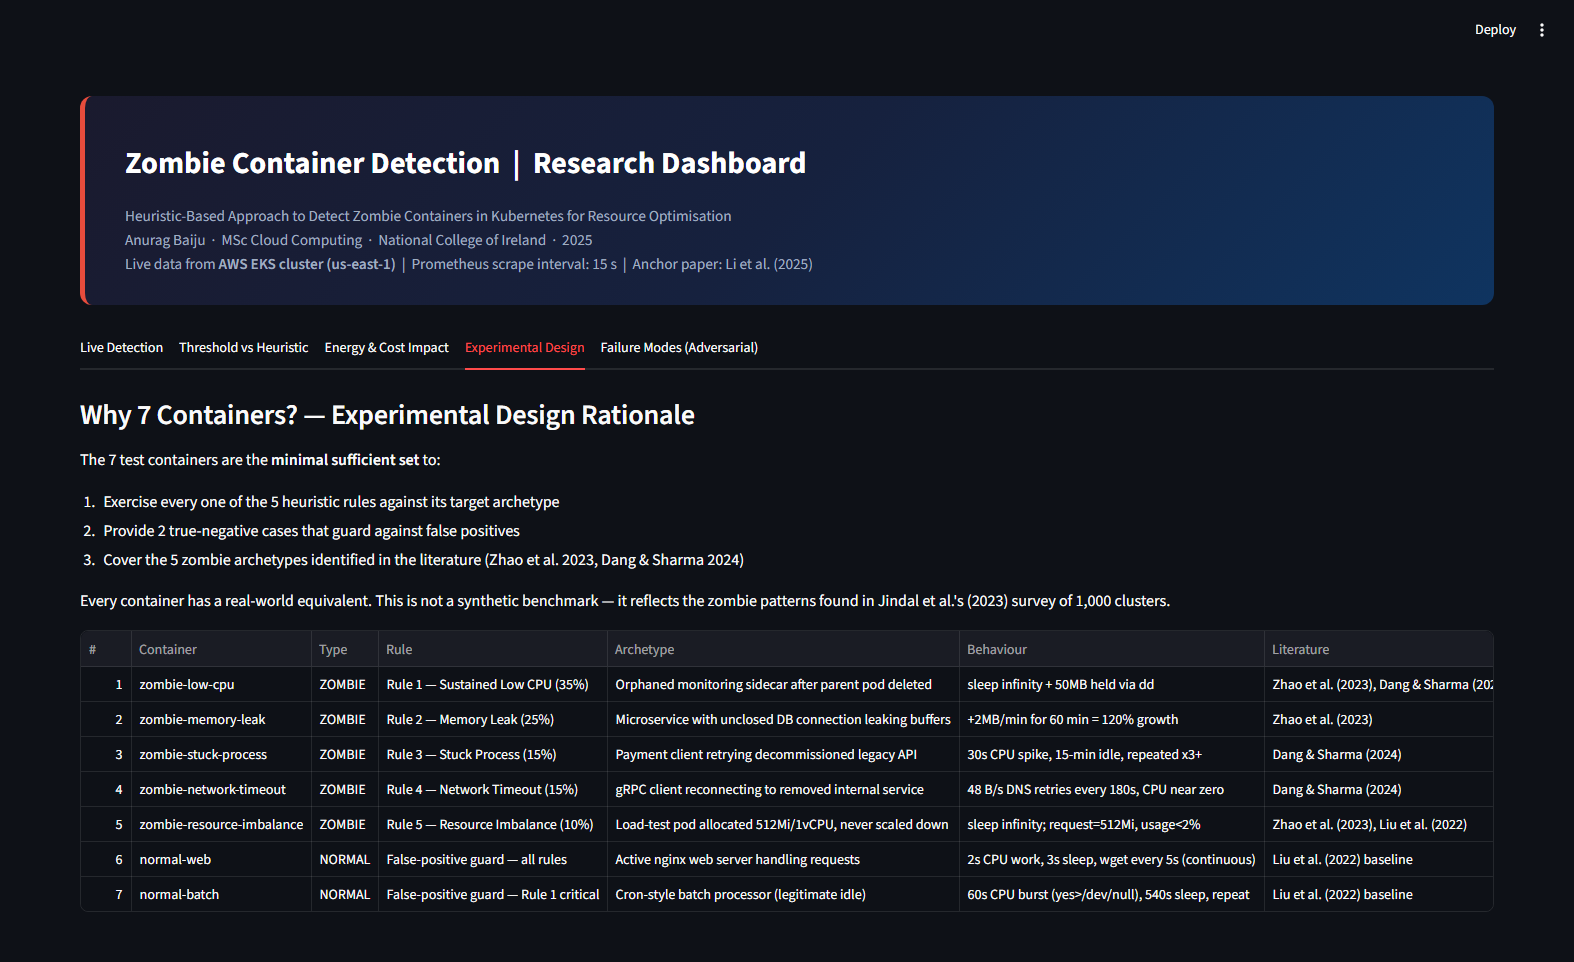
\includegraphics[width=\textwidth]{fig06_dashboard_experimental_design.png}
\caption{Dashboard Tab 4, ``Experimental Design'': the seven canonical
test pods and their archetype mapping, plus the literature references
that motivated each archetype.}
\label{fig:dash-design}
\end{figure}

% =============================================================================
\section{Discussion}
\label{sec:discussion}

\subsection{What works}

The detector achieves perfect recall on real zombies. Every container
known to the test ground truth as a zombie is flagged. This includes
the \texttt{adversarial-stealth-zombie} pod, which was constructed to
evade Rule~1 by injecting a five-second saturating CPU burst every
twelve minutes. The probe was successful at avoiding Rule~1 (the
spike-exclusion guard correctly fires), but Rule~3 caught the resulting
spike-then-idle pattern, and the rule's contribution to the composite
was sufficient to push the score above the zombie threshold.

The audit trail makes every decision inspectable. The exact metric
values that produced each rule score are written to the detector log
and exported as Prometheus gauges, which means an engineer can both
review historical decisions and write alerting rules on the
detector's own metrics.

The deployment fits inside the AWS free tier on ARM nodes. The detector
pod has accumulated more than five hours of uptime on
\texttt{t4g.small} hardware (one virtual CPU, two gigabytes of memory)
without restart, throttling or out-of-memory events. The single-process
design avoids the operational footprint that a graph-database-backed or
machine-learning-backed alternative would impose.

\subsection{What does not work}

The cost of one-hundred-per-cent recall is a fifty-per-cent false-positive
rate. Three of the five adversarial probes
(\texttt{adversarial-jvm-warmup}, \texttt{adversarial-cold-standby} and
\texttt{adversarial-low-traffic-api}) produced false positives on the
live cluster. None of these false positives is a bug in the
implementation; each one is an inherent boundary condition of behavioural
zombie detection.

\paragraph{JVM-style cache warmup.}
Memory that grows monotonically with no CPU activity has the same shape
as a leak. Any rule based on memory growth and low CPU will fire during
the warmup window. The mitigation is to consult pod uptime and
re-evaluate after the warmup period has had a chance to plateau, which
the current implementation does not do.

\paragraph{Cold standby.}
A pod that holds memory and emits keepalive heartbeats is
behaviourally identical to a network-timeout zombie. Disambiguation
requires an out-of-band signal, such as a pod annotation
(\texttt{zombie-detector.io/standby=true}) or correlation with
service-mesh request rate, neither of which the current detector
consumes.

\paragraph{Low-traffic real API.}
A real internal microservice that receives one request every five
minutes produces sustained low-volume network traffic with low CPU,
which is exactly the Rule~4 signature. Without an
application-layer signal (HTTP request count, gRPC success rate, or
similar), behavioural metrics alone cannot tell this apart from a
zombie that is retrying a decommissioned upstream.

\subsection{Trade-offs in summary}

Table~\ref{tab:tradeoffs} summarises the gains and losses delivered by
the design.

\begin{table}[H]
\centering
\caption{Trade-offs introduced by the heuristic design.}
\label{tab:tradeoffs}
\small
\begin{tabularx}{\textwidth}{lXX}
\toprule
\textbf{Property}        & \textbf{Gain}                                     & \textbf{Cost} \\
\midrule
Interpretability         & Per-rule scores with exact metric values          & --- \\
Operational overhead     & 100\,m CPU, 256\,Mi memory, single Python pod     & --- \\
Training data            & None                                              & Thresholds are global, not per-workload \\
Recall on idle zombies   & 100\,\%                                           & 50\,\% FPR on legitimately idle work \\
Coverage of duty cycle   & Rules 1, 3 and 5 use 60-min windows               & Cron jobs longer than the window are flagged \\
Application-layer aware  & ---                                               & Cannot disambiguate cold standby from retry-loop zombie \\
Adversarial robustness   & ---                                               & A determined attacker can defeat Rule 1 with synthetic spikes \\
Causal action            & Detection feeds an external scaler                & Detection alone does not save resources; an external system must act \\
\bottomrule
\end{tabularx}
\end{table}

\subsection{Why the seventy-five-per-cent number is the right one to report}

The original test set, comprising five canonical zombies and two
normals, scored one hundred per cent on every metric. The supervisor's
review correctly observed that this number was a function of the test
design rather than a measurement of the system: each test container was
constructed to match exactly one rule, and no test container was
constructed to defeat one. The five adversarial probes added in response
to this critique drove the combined accuracy down to seventy-five per
cent, and the failure-positive rate up from zero to fifty per cent. This
is the operational reality of a behavioural detector. The lower number
is the truthful one.

% =============================================================================
\section{Conclusion and Future Work}
\label{sec:conclusion}

The work has produced a five-rule heuristic detector for zombie
containers in Kubernetes, deployed it on Amazon EKS, and evaluated it
on a twelve-container test set that includes adversarial probes designed
to defeat its rules. The detector achieves seventy-five per cent
accuracy and one-hundred-per-cent recall, with three documented false
positives that arise from the inherent ambiguity of behavioural metrics
in the absence of application-layer signal.

The work positions itself as the missing classification layer of
Li et al.'s (2025) Energy-Aware Elastic Scaling Algorithm. EAES assumes
a list of zombies as input. The detector produces that list, with an
audit trail that allows an SRE to verify each entry before it is fed
into a scaling decision. The energy quantification in this report
re-uses Li et al.'s power formula on a per-container basis, completing a
chain from \emph{detect} (this work) to \emph{quantify} (the energy
formula) to \emph{act} (EAES).

\subsection{Limitations}

The thresholds are global rather than per-workload; a mixed estate
running Java microservices alongside short-lived Python lambdas would
benefit from per-namespace overrides, which the current implementation
does not support. The analysis window is fixed at sixty minutes, which
makes the detector blind to workloads with duty cycles longer than that.
Reading Kubernetes \texttt{CronJob} schedules and adapting the window
per pod would close this gap.

\subsection{Future work}

Three directions are immediately actionable. First, an
application-layer corroboration step that consults a service-mesh
request count before classifying a low-network container as a Rule~4
zombie would eliminate the false positive on
\texttt{adversarial-low-traffic-api} and on real low-traffic APIs in
production clusters. Second, a pod-annotation system
(\texttt{zombie-detector.io/standby=true},
\texttt{zombie-detector.io/window-minutes=180}) would let operators
opt specific pods out of specific rules, addressing the cold-standby
false positive. Third, layering an isolation-style anomaly detector on
top of the rule engine, combined via a small meta-classifier, would
catch stealth zombies that have learned to evade Rule~1, at the cost of
introducing a small training requirement.

\subsection{Practical advice for the reviewer}

The cluster used for this evaluation is still running. The
\texttt{show\_evidence.ps1} PowerShell script in the repository runs the
nine commands behind Figures~\ref{fig:nodes-cli} through~\ref{fig:prom},
pausing between each so that the reader may verify the live state for
themselves. The Streamlit dashboard runs locally and renders the same
metrics that the figures above show.

\begin{figure}[H]
\centering
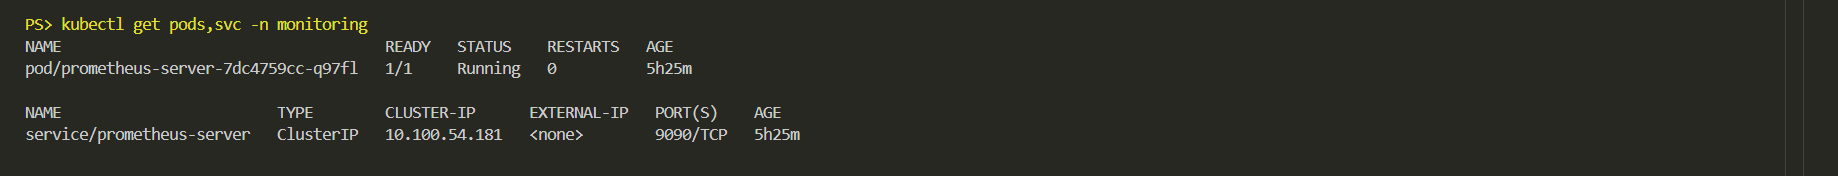
\includegraphics[width=\textwidth]{fig18_terminal_prometheus.png}
\caption{Final live verification: Prometheus pod and service in the
\texttt{monitoring} namespace, after more than five hours of uptime.}
\label{fig:prom}
\end{figure}

% =============================================================================
\begin{thebibliography}{9}

\bibitem{li2025}
H.~Li, W.~Rao, B.~Hu, Y.~Tian, and J.~Shen.
\newblock Energy-Aware Elastic Scaling Algorithm for Kubernetes Microservices.
\newblock \emph{Journal of Network and Computer Applications}, Elsevier, 2025.

\bibitem{jindal2023}
A.~Jindal, M.~Chadha, S.~Benedict, and M.~Gerndt.
\newblock Characterising Resource Usage Patterns in Kubernetes
Production Clusters.
\newblock In \emph{Proceedings of the 2023 IEEE International Conference
on Cloud Engineering}, IEEE, 2023.

\bibitem{stormforge2021}
StormForge.
\newblock Cloud Optimisation Survey 2021: The State of Kubernetes
Resource Waste.
\newblock Industry report, 2021.

\bibitem{kubernetes-cadvisor}
The Kubernetes Authors.
\newblock cAdvisor metrics reference, kubelet built-in metrics endpoint.
\newblock \url{https://kubernetes.io/docs/concepts/cluster-administration/system-metrics/}, accessed 2026.

\bibitem{prometheus-docs}
Prometheus Authors.
\newblock Prometheus documentation: scrape configuration, PromQL,
\texttt{prometheus\_client} library.
\newblock \url{https://prometheus.io/docs/}, accessed 2026.

\bibitem{eksctl-docs}
Weaveworks.
\newblock \texttt{eksctl} The official CLI for Amazon EKS.
\newblock \url{https://eksctl.io/}, accessed 2026.

\end{thebibliography}

% =============================================================================
\appendix
\section{Repository layout}
\label{app:layout}

The supplementary material accompanying this report includes the
following items, all available in the project repository.

\begin{description}[leftmargin=2em,style=nextline]
\item[\texttt{src/}] Python source for the detector
(\texttt{heuristics.py}, \texttt{detector.py},
\texttt{metrics\_collector.py}, \texttt{exporter.py},
\texttt{energy\_impact.py}, \texttt{evaluation.py}, \texttt{main.py}).
\item[\texttt{kubernetes/}] All deployment manifests
(namespaces, RBAC, Prometheus, the twelve test scenarios, the
detector with its ConfigMap-mounted source).
\item[\texttt{dashboard/}] Streamlit application source.
\item[\texttt{images/}] Eighteen figures referenced in this report,
indexed \texttt{fig01\_*} through \texttt{fig18\_*}.
\item[\texttt{evaluation\_results.json}, \texttt{.csv}] Live measured
results of the evaluation in Section~\ref{sec:evaluation}.
\item[\texttt{generate\_architecture\_diagram.py}] Reproduces
\texttt{fig01\_system\_architecture.png}.
\item[\texttt{capture\_report\_images.py}] Selenium-driven
re-capture of the dashboard tabs and the Prometheus targets page.
\item[\texttt{show\_evidence.ps1}] PowerShell script that runs the
nine \texttt{kubectl} commands referenced in
Section~\ref{sec:evaluation}, with a pause between each so that
screenshots can be taken cleanly.
\item[\texttt{PROFESSOR\_RESPONSE.md}] Point-by-point response to the
supervisor's review, mapping each piece of feedback to the file or
figure that addresses it.
\end{description}

\end{document}
